\documentclass[sigconf,review, anonymous]{acmart}
\acmConference[ESEC/FSE 2019]{The 27th ACM Joint European Software Engineering Conference and Symposium on the Foundations of Software Engineering}{26--30 August, 2019}{Tallinn, Estonia}

\usepackage{booktabs} % For formal tables
%\usepackage{backnaur}
\usepackage{syntax}
\usepackage{calc}
\usepackage{listings}
\usepackage{url}
\usepackage{color}
\usepackage{graphicx}
%\usepackage{subcaption}
\usepackage{subfig}
\captionsetup{compatibility=false}
\usepackage{amssymb,proof}
\usepackage[]{algorithm2e}

\lstset{frame=tb,
  language=Java,
  aboveskip=3mm,
  belowskip=3mm,
  showstringspaces=false,
  columns=flexible,
  basicstyle={\small\ttfamily},
  numbers=left,
  breaklines=true,
  breakatwhitespace=true,
  tabsize=3,
   stepnumber=1,
}
%\newenvironment{bnfsplit}[1][0.7\textwidth]
%{\minipage[t]{#1}$}
%{$\endminipage}


%\renewcommand{\baselinestretch}{0.945}
%\newcommand*\samethanks[1][\value{footnote}]{\footnotemark[#1]}

% Copyright
%\setcopyright{none}
% \setcopyright{acmcopyright}
%\setcopyright{acmlicensed}
% \setcopyright{rightsretained}
%\setcopyright{usgov}
%\setcopyright{usgovmixed}
%\setcopyright{cagov}
%\setcopyright{cagovmixed}


% DOI
% \acmDOI{10.475/123_4}

% ISBN
% \acmISBN{123-4567-24-567/08/06}

%\acmPrice{15.00}

\newcommand{\unit}{ ( ) }
\newcommand{\rn}[1]{\scriptscriptstyle\mathtt{#1}}
\newcommand{\compose}[2]{#1 \; ; \; #2}
\newcommand{\return}[1]{return\: #1}
\newcommand{\throw}[1]{throw\: #1}
\newcommand{\ifr}[3]{if \; #1 \; then \; #2 \; else \: #3}
\newcommand{\rstate}[2]{#1 \:;\: #2}
\newcommand{\step}[5]{\rstate{#1}{#2}\ \mapsto_{#5}\ \rstate{#3}{#4}}
\newcommand{\sstep}[3]{#1\: \mapsto_{#2}\: #3}
\newcommand{\lookup}[2]{#1(#2)}
\newcommand{\sub}[3]{[#1/#2]#3}


\begin{document}

\newcommand{\mike}[1]{\textcolor{red}{#1}}
\newcommand{\vaibhav}[1]{\textcolor{red}{#1}}
\newcommand{\soha}[1]{\textcolor{red}{#1}}
\newcommand{\smcc}[1]{\textcolor{red}{#1}}

\newcommand{\toolshort}{JR}
\newcommand{\tool}{Java Ranger}
\newcommand{\toolfull}{Java Ranger}

\title{\tool: Static Regions for Efficient Symbolic Execution of Java}

\author{Vaibhav Sharma}
\authornote{Both authors contributed equally to this research.}
\email{vaibhav@umn.edu}
\author{Soha Hussein}
\authornotemark[1]
\email{husse200@umn.edu}
\affiliation{%
\institution{University of Minnesota}
\city{Minneapolis}
\state{MN}
\postcode{55455}
\country{USA}
}

\author{Michael W. Whalen}
\affiliation{%
\institution{Amazon Web Services}
\city{Minneapolis}
\state{MN}
\country{USA}}
\email{mww@amazon.com}

\author{Stephen McCamant}
\affiliation{%
\institution{University of Minnesota}
\city{Minneapolis}
\state{MN}
\postcode{55455}
\country{USA}
}
\email{smccaman@umn.edu}

\author{Willem Visser}
\affiliation{%
\institution{Computer Science Division, University of Stellenbosch}
\city{Stellenbosch}
\country{South Africa}}
\email{wvisser@cs.sun.ac.za}

\maketitle
\begin{abstract}

%Scaling symbolic execution to industrial-sized programs is an important open research problem.  Veritesting introduced bounded static regions in symbolic execution to improve scalability by combining the advantages of static symbolic execution with those of dynamic symbolic execution.  Bounded static regions reduce the number of paths to explore in symbolic execution by describing regions of code using disjunctive formulas.
%%
%In previous work, veritesting was applied to binary-level symbolic execution.

%Integrating veritesting with Java bytecode presents unique challenges, 
%notably, incorporating many more non-local control jumps caused by runtime polymorphism, exceptions, native calls, and dynamic class loading.
%%
%If these languages features are not accounted for, the static code regions described by veritesting are often small and may not lead to substantial reduction in paths.  In addition, the use of disjunctive regions forces previously concrete assignments to become symbolic leading to additional solver calls.  

%In this paper, we describe \tool, which adds static regions to Java Symbolic Pathfinder.  Unlike previous approaches, it adds support for {\em higher order} Veritesting regions into which we can instantiate static regions for staticly- and dynamically-dispatched function calls.  Although our tool is still an unoptimized prototype, we show that it dramatically outperforms Java Symbolic Pathfinder on a number of benchmark examples, and that support for higher-order regions substantially improves the performance of Veritesting for Java programs.

Merging related execution paths is a powerful technique for reducing
path explosion in symbolic execution.
%
One approach, introduced and dubbed ``veritesting'' by Avgerinos et
al., works by statically translating a bounded control flow region
into a single formula.
%
This approach is a convenient way to achieve path merging as a
modification to a pre-existing single-path symbolic execution engine.
%
Avgerinos et al. evaluated their approach in a symbolic execution tool
for binary code, but different design considerations apply when
building tools for other languages.
%
In this paper we explore the best way to use a veritesting approach in
the symbolic execution of Java.

Because Java code typically contains many small dynamically dispatched
methods, it is important to include them in veritesting regions; we
introduce a {\em higher-order} veritesting technique to do so
modularly.
%
Java's typed memory structure is very different from a binary, but we
show how the idea of static single assignment (SSA) form can be
applied to object references to statically account for aliasing.
%
More formally, we describe our veritesting algorithms as
syntax-directed transformations of a structured intermediate
representation, which highlights their logical structure.
%
We have implemented our algorithms in \tool, an extension to the
widely used Symbolic Pathfinder tool for Java bytecode.
%
Our empirical evaluation shows that veritesting greatly reduces the
search space of Java symbolic execution benchmarks, while our expanded
capabilities provided a significant further improvement.



\end{abstract}

%\keywords{multi-path symbolic execution; veritesting; Symbolic
%PathFinder; static analysis}


%Path explosion problem is still the main obsticale against scaling up symbolic execution to industrial sized projects.
%%
%One interesting resolution to the problem is \emph{Veritesting}, which represents regions of code as disjunctive formals over paths.
%%
%Unlike the C compiler that inlines functions in programs, Integrating veritesting with Java bytecode presents unique challenges: notably, incorporating non-local control jumps caused by runtime polymorphism, exceptions, native calls, and dynamic 3 class loading.
%%
%In this paper we present our robust implementation of Java based veritesting tool that supports dynamic dispatch and
\section{Introduction}
%
Symbolic execution is a popular analysis technique that performs non-standard execution of a program: data operations generate formulas over inputs, and  branch constraints along an execution path are combined into a predicate.
%
Originally developed in the 1970s~\cite{King1976,Clarke1976}, symbolic execution is a convenient building block for
program analysis, since arbitrary query predicates can be combined with the logical program representation, and
solutions to these constraints are program inputs illustrating the queried behavior.
%
Some of the applications of symbolic execution include
test generation~\cite{dart,cute}, equivalence checking~\cite{ramos,adaptorsynth}, vulnerability finding~\cite{driller,angr}, and protocol correctness checking~\cite{transport}.
%
Symbolic execution tools are available for many languages, including
CREST~\cite{BurnimS2008} for C source code, KLEE~\cite{CadarDE2008}
for C/C++ via LLVM, JDart~\cite{jdart2016} and Symbolic
PathFinder (SPF)~\cite{spf} for Java, and S2E~\cite{ChipounovKC2012},
FuzzBALL~\cite{BabicMMS2011}, and {\tt angr}~\cite{angr} for binary code.
%
%Some of these tools, such as {\tt angr} and Mayhem~\cite{mayhem} that operate at the binary-level, are used for finding
%security bugs.
%
%Others, such as KLEE, are used for exploring system-level programs for software engineering purposes.

% \mike{More here...explain the `ecosystem' - tools for different languages: KLEE, FuzzBall, Java Symbolic Pathfinder, ...}

Although symbolic analysis is a popular technique, scalability is a substantial challenge for many applications.
%
In particular it can suffer from a {\em path explosion}: complex
software has exponentially many execution paths, and baseline symbolic
execution techniques that explore one path at a time are unable to
cover all paths.
%
Dynamic state merging~\cite{HansenSS2009,kuznetsov} provides one way to
alleviate scalability challenges by opportunistically merging dynamic
symbolic executors, effectively merging the paths they represent.
%
Avoiding even a single branch point can provide a multiplicative
savings in the number of execution paths, though at the potential cost
of making symbolic state representations more complex.

 %, which can be performed on paths or even on environments~\mike{FM paper from 2014 on Javascript?}., not sure what Mike meant to say here - Vaibhav % He may have meant MultiSE? - Stephen
%
%Other techniques such as subsumption checking~\cite{Tian:2017:MEI:3155562.3155589} make use of interpolants to find
%guarantees about safety properties on an execution path.
 
%
Veritesting~\cite{veritesting} is another recently proposed technique that can dramatically improve the performance of symbolic execution by effectively merging paths.  Rather than explicitly merging state representations, veritesting encodes a local region of a program containing branches as a disjunctive region for symbolic analysis. This often allows many paths to be collapsed into a single path involving the region.  
%
In previous work~\cite{veritesting}, constructing bounded static code regions was shown to allow symbolic execution to find more bugs, and achieve more
node and path coverage, when implemented at the X86 binary level for compiled C programs.
%
This motivates us to investigate using static regions for symbolic execution of Java software (at the Java bytecode level).

Java programmers who follow best software engineering practices attempt to write code in an object-oriented
form with common functionality implemented as a Java class and multiple not-too-large methods used to implement small
sub-units of functionality.
%
This causes Java programs to make several calls to methods, such as getters and setters, to re-use small common sub-units
of functionality.
%
Merging paths within regions in such Java programs using techniques described in current literature is limited by not having the ability
to inline method summaries.
%
This is not a major impediment for compiled C code, as the C compiler will usually automatically inline the code for short
methods such as \texttt{get}.
%
However, Java has an {\em open world} assumption, and most methods are {\em dynamically dispatched}, meaning that the code to be
run is not certain until a method is resolved at runtime; if inlining is performed at all, it is by the JRE, so it is not reflected in bytecode.

Not being able to summarize such dynamically dispatch methods can lead to poor performance for
n\"aive implementations of bounded static regions.
%
Thus, to be successful, we must be able to inject the static regions associated with the calls into the dispatching
region.
%
We call such regions {\em higher order} as they require a region as an argument and can return a region that may need
to be further interpreted.
%
In our experiments, we demonstrate exponential speedups on benchmarks (in general, the more paths contained within a
program, the larger the speedup) over the unmodified Java SPF tool using this approach.

Another common feature of Java code that represents the boundary of path merging is \textit{exceptions}.
%
If an exception can potentially be raised in a region, the symbolic executor needs to explore that exceptional behavior.
%
But, it is possible for other unexceptional behavior to also exist in the same region.
%
For example, it can be in the form of a branch nested inside another branch that raises an exception on the other side.
%
Summarizing such unexceptional behavior while simultaneously guiding the symbolic executor towards potential exceptional
behavior reduces the branching factor of the region.
%
We propose a technique named \textit{Single-Path Cases} for splitting a region summary into its exceptional and
unexceptional parts.

While summarizing higher-order regions and finding single-path cases is useful to improve scalability,
representing such summaries in an intermediate representation~(IR) that uses static single-assignment~(SSA) form
provides a few key advantages.
%
(1) It allows region summaries to be constructed by using a sequence of transformations, with each transformation
extending to add support for new features such as heap accesses, higher-order regions, and single-path cases.
%
(2) It allows for simplifications such as constant propagation, copy propagation, constant folding to be performed on
region summaries.
%
(3) It makes the construction of region summaries more accessible to users of the symbolic execution tool, thereby making
path merging more useful to end-users.\\
%
In this paper, we present Java Ranger, an extension of Symbolic PathFinder, that computes such region summaries over a representation we call
Ranger IR.
%
Ranger IR has support for inlining method summaries and for constructing SSA form for heap accesses.
%
It also proposes Single-Path Cases as an alternative to multiple transition points as
defined by Avgerinos et al.~\cite{veritesting}.

This paper extends our initial investigations of Java veritesting
reported in a paper at the 2017 JPF
workshop~\cite{sharma-veritesting}.
%
Our workshop paper motivated some of the ways in which Java
veritesting is different from veritesting for binary code and the
value that veritesting could provide, but it did not describe an
end-to-end automated implementation.
%
The present paper describes a number of conceptual improvements that
are new since the workshop paper, including the Ranger IR, single-path
cases, and the details of our higher-order region approach.
%
We have also made a number of architectural changes, such as switching
from Soot to Wala for static analysis and using Green for formula
representation, and we have integrated \tool\ as an extension to SPF
and evaluated it in several case studies.

\subsection{Motivating Example}
\begin{figure*}
    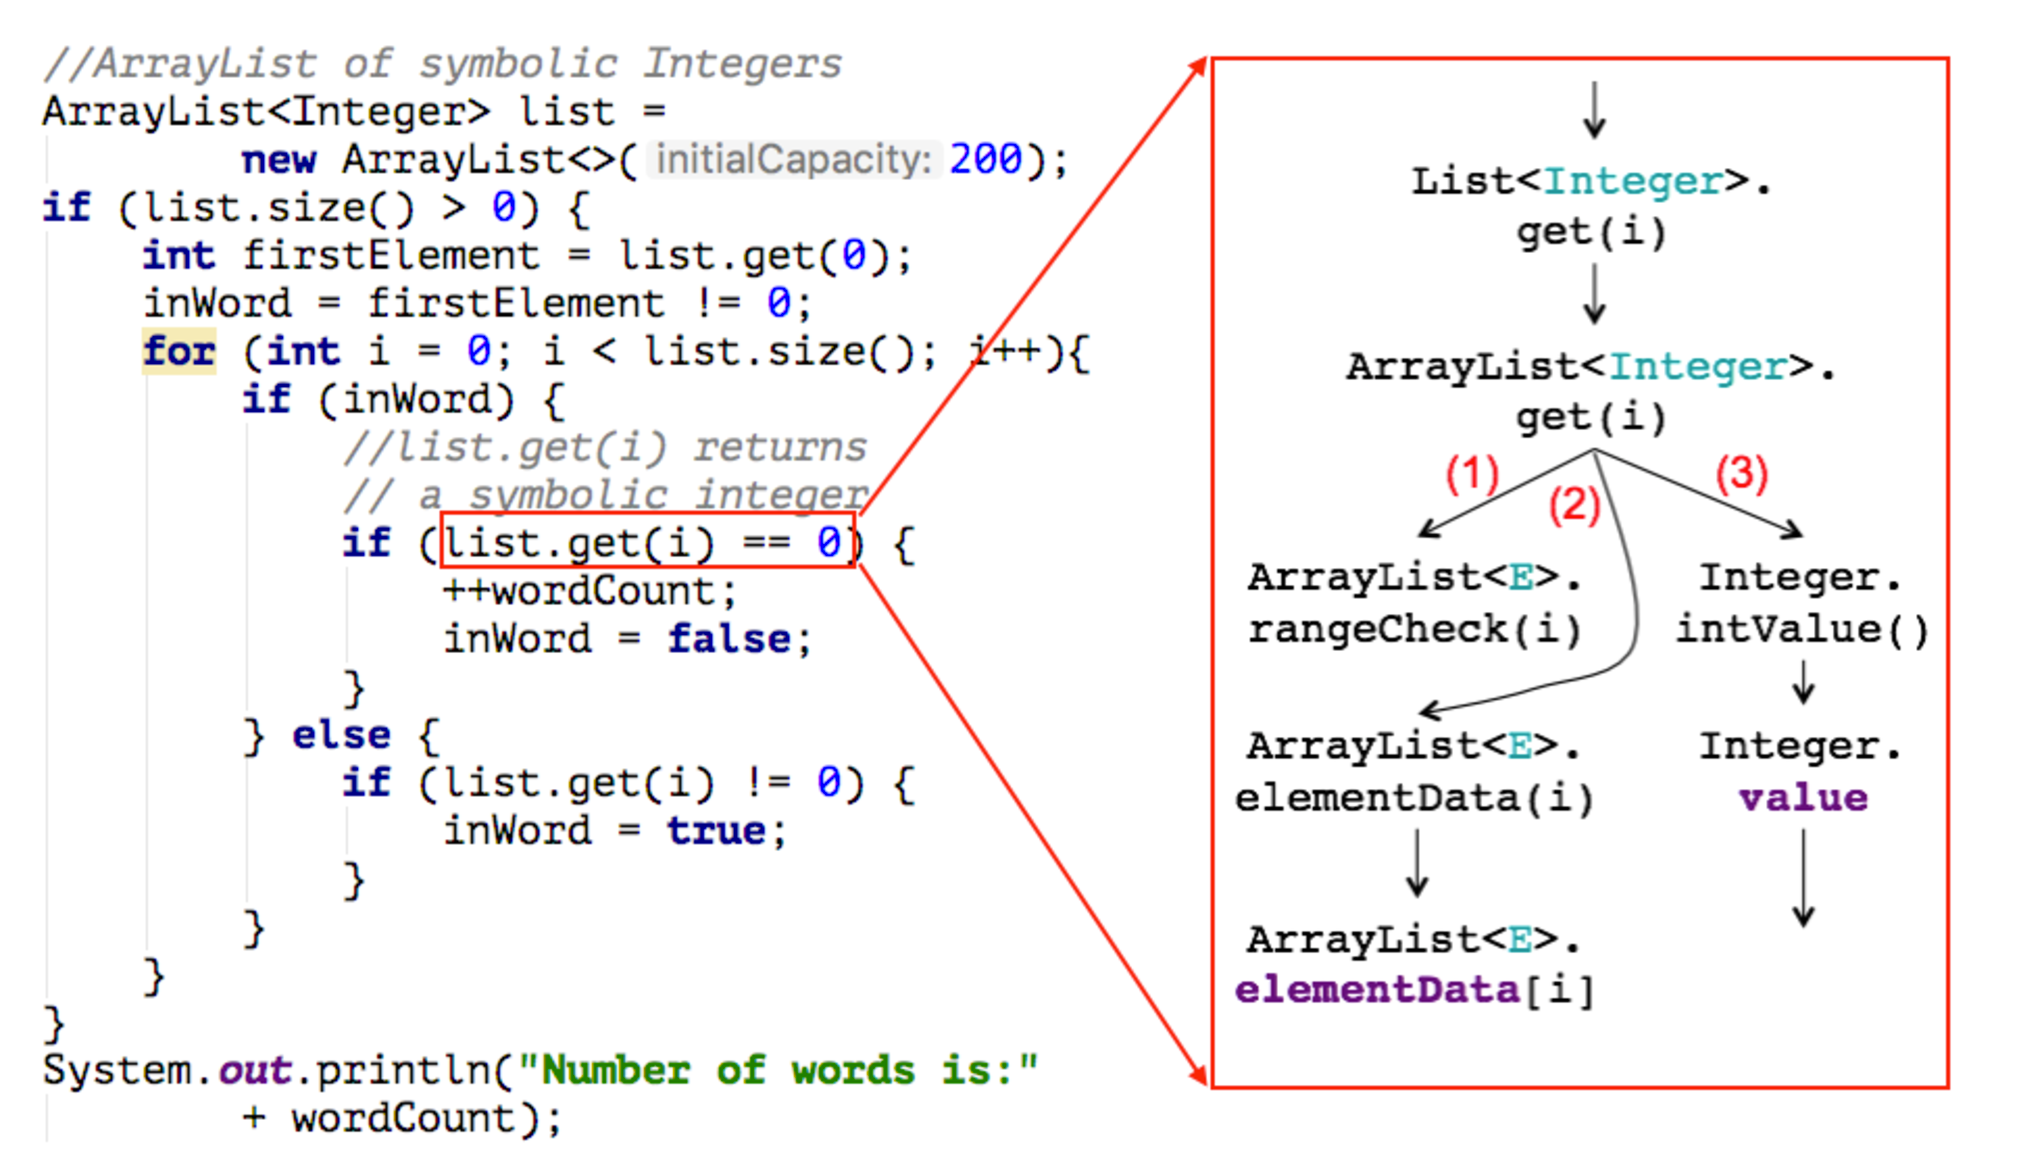
\includegraphics[width=0.8\textwidth]{figures/wordCount.pdf}
    \caption{An example demonstrating the need for using a multi-path region summary}
    \label{fig:mot-example}
\end{figure*}
Consider the example of Java code shown in Figure \ref{fig:mot-example}.
%
The {\tt list} object refers to an {\tt ArrayList} of 200 {\tt Integer} objects which have an unconstrained symbolic
integer as a field.
%
The checking of each even-indexed entry in {\tt list} introduces a branch, which has both sides feasible, and requires
symbolic execution to explore two execution paths instead of the one it was at.\\
%
Performing this check over the entire {\tt list} makes symbolic execution need $2^{100}$ execution paths to terminate
(assuming {\tt list} has 200 entries with every even-indexed entry pointing to a new unconstrained symbolic integer).
%
A simple way to avoid this path explosion is to merge the two paths arising out of the {\tt i\%2 == 0 \&\& list.get(i) == 42} branch.
%
Such path merging requires us to compute a summary of all behaviors arising on both sides of the branch from lines 11 to 13
until both sides of the branch merge at line 14.
%
If we can construct such a summary beforehand, our symbolic executor can instantiate the summary by reading in inputs to
the summary from the stack and/or the heap, and writing outputs of the summary to the stack and/or the heap.\\
%
Unfortunately, constructing such a summary for this simple region from lines 11--13 is not straightforward due to the
call to {\tt list.get(int)} which is actually a call to {\tt ArrayList<Integer>.get(int)} ({\tt java.util.List<E>.get(int)} is abstract and does not have an implementation).
%
{\tt ArrayList<Integer>.get(int)} internally does the following:
%
\begin{enumerate}
\item It checks if the index argument accesses a value within bounds of the {\tt ArrayList} by calling {\tt ArrayList<E>.rangeCheck(int)}. If this access is not within bounds, it throws an exception.
%
\item It calls {\tt ArrayList<E>.elementData(int)} to access an internal array named {\tt elementData} and get the entry at position {\tt i}. This call results in an object of class {\tt Integer} being returned.
%
\item It calls {\tt Integer.intValue()} on the object returned by the previous step. This call internally accesses the {\tt value} field of {\tt Integer} to return the integer value of this object.
%
\end{enumerate}

The static summary of {\tt ArrayList<Integer>.get(int)} needs to not only include summaries of all these three methods but
also include the possibility of an exception being raised by the included summary of {\tt ArrayList<E>.rangeCheck(i)}.
%
Our extension to path-merging includes using method summaries, either with a single return or no return, as part of region summaries that have method calls \footnote{We plan to support methods with multiple returns in the future.}.
%
The method whose summary is to be included depends on the dynamic type of the object reference on which the method is being invoked.
%
In our example, the dynamic type of {\tt list} is {\tt ArrayList}, whereas it is declared statically as having the type {\tt List}.
%
Therefore, the summary of {\tt list.get(i)} pulls in the method summaryof {\tt ArrayList<E>.get(i)}.\\
%
Our \textit{Single-Path Cases} extension to path-merging also allows the possibility of exceptional behavior being
included in the summary and explored separately from unexceptional behavior by performing exploration of exceptional
behavior in the region on its own execution path.
%

%\section{Preliminaries}
\mike{KEEP?}

In this section, we describe the different technologies that are used to construct \tool.  

\subsection{SPF}
Symbolic PathFinder (SPF) \cite{spf} combines symbolic execution with model checking and constraint solving for test case generation. In this tool, programs are executed on symbolic inputs representing multiple concrete inputs. Values of variables are represented as numeric constraints, generated from analysis of the code structure. These constraints are then solved to generate test inputs guaranteed to reach that part of code. Essentially SPF performs symbolic execution for Java programs at the bytecode level. Symbolic PathFinder uses the analysis engine of the NASA Ames JPF model checking tool (i.e. jpf-core) \cite{jpf}.


\subsection{WALA and SSA Form}
In order to find the static regions that we compile into disjunctive predicates, we use the open-source WALA library~\cite{}.  WALA can construct several different intermediate representations from Java bytecode including single-static assignment (SSA) form~\cite{}.  The SSA form is particularly attractive for constructing static regions as (for loopless code) there is a unique variable for each assignment, affording a straightforward translation into a predicate representing the region.  

We chose WALA specifically over competing solutions such as Soot~\cite{} because it maintains the bytecode offset of statements and the stack locations of local variables used in the SSA form.  This allows us to easily interface with the existing SPF code, by binding (through equalities) the symbolic or concrete values stored on the stack for inputs and also to store the variables corresponding to final values of computed variables back onto the stack.

\iffalse
\subsection{WALA/CFG/SSA Form}
...something here on WALA

%\subsection{CFG}
A control flow graph (CFG) in computer science is a representation, using graph notation, of all paths that might be traversed through a program during its execution.
In a control flow graph each node in the graph represents a basic block, i.e. a straight-line piece of code without any jumps or jump targets; jump targets start a block, and jumps end a block. Directed edges are used to represent jumps in the control flow. There are, in most presentations, two specially designated blocks: the entry block, through which control enters into the flow graph, and the exit block, through which all control flow leaves.


\subsection{Veritesting}
Veritesting\cite{veritesting} is a technique that reduces the number of paths that need to be explored by avoiding unnecessary forking.
%
Veritesting identifies regions of if-statements that can be statically explored and captured in a logical formula (usually as disjunction of formulas representing different branches in if-statement).
%
We will call this formula VeriFormula which captures possible different execution paths.
%
The result of this process is a VeriFormula, which can be submitted to a SMT solver.
%
If the formula is satisfiable, then there is some path through the code region that reaches the exit point. In this case, dynamic symbolic execution is resumed after updating the PC with the VeriFormula and also updating symbolic values of variable if needed.
\fi


%\section{Challenges}

While the performance improvement demonstrated on the code in Listing 1 is impressive, it is perhaps not representative of most Java code.  Java conventions encourage the use of indirection when accessing class fields using non-static {\em get} and {\em set} methods, as well as liberal use of exceptions.  Unlike C compilers, which assume a ``closed world'' and often inline simple functions into the body of calling methods to improve performance, the Java compiler must assume an ``open world'' in which a class may be used in a new context, so inlining of non-final methods is unsafe.

Previous approaches to veritesting exit static code regions when indirect calls to functions or non-local jumps are made.  In this section, we explore how the structure of Java programs reducees the performance of a n\"aive veritesting approach.

%Talk about how veritesting is different when done on Java bytecode
%
%The transition points at the Java bytecode level are return, exceptions (done using athrow), virtual function invocations (invokevirtual, invokeinterface), native calls (also done using invokevirtual), reflection and dynamic class loading (also done using invokevirtual).
%
%Present results from Soot-based static analysis
%
%Talk about how veritesting gets harder to do when considering multi-threaded Java bytecode.
\subsection{Exit Points}
\label{sec:exit_points}

\mike{Should we re-run this analysis with WALA for consistency's sake?}
%While the performance improvement shown in Figure~\ref{fig:v_ex_plot} with statically unrolling the three-way branches is clear, we need to automate this process.
%
Integrating veritesting with SPF requires that we can represent a region of a Java program as a disjunctive formula with multiple exit points.  Each exit point describes a possible distinct continuation of the current path after the static code region completes execution.  Avgerinos et al.~\cite{veritesting} defined exit points as unresolved jumps, function boundaries, and system calls.
%
These exit points are nodes in a control-flow graph which represent non-local control flow, and therefore, need to be explored using plain dynamic symbolic execution.
%
In the context of Java bytecode, we find such non-local control flow in five ways listed as follows: (1) return statements, (2) exceptions, (3) virtual function invocations~(\textit{invokevirtual}, \textit{invokeinterface}), (4) reflection, (5) native calls.
%
\iffalse
\mike{These explanations are obvious and can be dispensed with if we need space}
Return statements form the function boundary, and are obvious candidates to be considered as exit points.
%
Exceptions are used to catch unexpected behavior, and often help design of cleaner code, and allow developers to capture useful information when such errors occur.
%
Virtual function invocations occur due to runtime polymorphism supported by Java.
%
The runtime environment binds the method call to its body by using the type of the object making the call.
%
Using reflection requires loading a class at runtime, identifying a method within the class, and calling it.
%
It is primarily used for extensibility purposes, achieving separate compilation, and generating a class at runtime.
\fi
%
%An approach such as Avgerinos et al.~\cite{veritesting} would force
%static code regions when any of these five constructs are encountered.

%Such regions must correctly preserve the semantics of symbolic execution for all possible Java constructs.
%
The primary benefit of implementing veritesting comes from its conversion of branches into disjunctions in a multi-path region.
%
But this benefit exists only when the number of different exit points from the disjunctive formula is less than the number of execution paths through the region in the first place.
%
For example, all execution paths in the first three-way branch in
Listing~\ref{lst:v_ex} joined together on line 7, causing the three-way branch to have a single exit point.
%
Therefore, it is crucial for us to study the number of exit points for each of our statically-analyzed regions vs. the number of branches within the region.
%
%
%Native calls are used to execute code outside of the Java Runtime Environment.
%
%Incorporating these into our static analysis would require handling virtual function invocations as well as static analysis of binary code.

These five types of exit points create the kind of non-local control flow which formed the frontier of the visible control-flow graph created as a result of \textit{CFGReduce} step by Avgerinos et al.
%
However, many of these exit points are used pervasively by Java developers.
%
For example, the Visitor design pattern is used extensively by the ASM framework~\cite{asm}, Soot~\cite{soot} and makes use of Java\rq s dynamic dispatch mechanism.
%
Running into exit points too often causes our statically-analyzed regions to be small and our performance gain from having fewer branches to be lost.

We investigated the occurrence of these exit points by creating a Soot-based static analysis of six large open-source projects written in Java.
%
Software faults from these six projects are maintained in the Defects4J~\cite{defects4j} repository.
%
We used Soot to create a control-flow graph for every method body in every class file in these six projects.
%
For each control-flow graph, we used nodes corresponding to conditional jump bytecodes as a starting point of our analysis.
%
We measured the number of instructions encountered when traversing down each side of the branch until we get to the immediate post dominator~\cite{dragon-book} of our starting point.
%
If there were no exit points encountered on any side of the branch, we considered this region as a pure multi-path region and calculated its size in bytecode instructions.
%
Finally, we allowed up to five nested branches and calculated the number of bytecode instructions from the earliest, as well as, the latest starting point in our control-flow graph traversal to an exit point.

As an example, we modify the three-way branch in Listing~\ref{lst:v_ex} by adding a {\tt else return;} to get the snippet shown in Listing~\ref{lst:v_ex_modified}.
%
\lstinputlisting[caption={Listing~\ref{lst:v_ex} modified to have a return statement in the three-way branch},
label={lst:v_ex_modified}, language=Java]{code_samples/VeritestingPerf_modified.java}
%
This results in bytecode that produces the control-flow graph shown in Figure~\ref{fig:v_ex_cfg}.
%
Nodes are numbered 1 through 6 with node (1) being the starting point and node (6) being the immediate post-dominator of node (1).
%
Nodes contain bytecode instructions along with instruction offsets.
%
The added \textit{return} statement creates an exit point, which causes the three-way branch in Listing~\ref{lst:v_ex_modified} to contain two exit points.
%
Counting the number of instructions after the {\tt ifge} instruction in node (1) through node (2) to node (6) gives us two instructions.
%
The same count going through nodes (3) and (4) to (6) gives us 6 instructions, and through nodes (3) to (5) gives us 4 instructions.
%
The presence of the \textit{return} statement in node (5) prevents this region from being a pure multi-path region.
%
\begin{figure}[]
\caption{Control-flow graph with {\tt else return;} added as line 7 of Listing~\ref{lst:v_ex}}
\label{fig:v_ex_cfg}
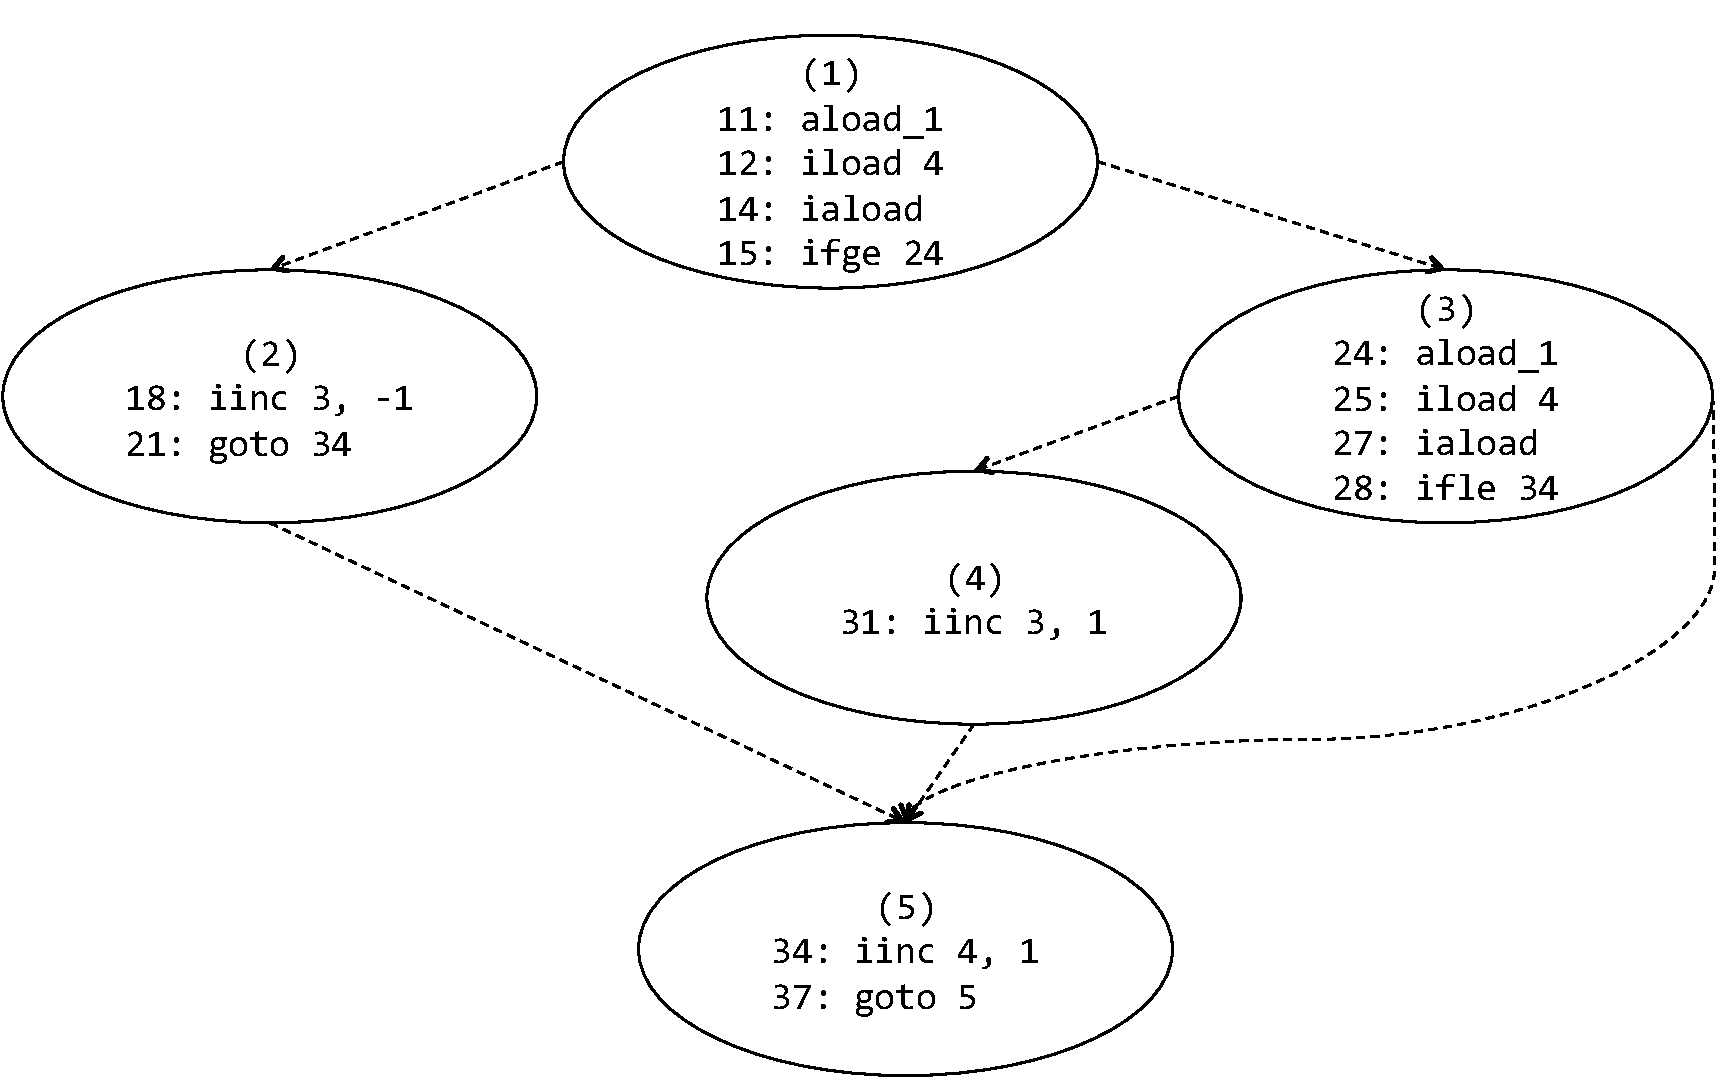
\includegraphics[width=\columnwidth]{figures/v_ex_cfg}
\end{figure}

%
We report our results from a Soot-based static analysis in Tables~\ref{t:r_s} and~\ref{t:r_c}.
%
\begin{table}[]
\centering
\begin{tabular}{|l|l|l|l|l|l|}
\hline
        & \#classes & \begin{tabular}[c]{@{}l@{}}if-\\ return\end{tabular} & \begin{tabular}[c]{@{}l@{}}if-\\ invokevirtual\end{tabular} & \begin{tabular}[c]{@{}l@{}}if-\\ throw\end{tabular} & \begin{tabular}[c]{@{}l@{}}region \\ size\end{tabular} \\ \hline
chart   & 679       & 8.44                                                 & 27.47                                                       & 4.33                                                & 13.59                                                  \\ \hline
closure & 1339      & 7.35                                                 & 22.1                                                        & 9.5                                                 & 11.66                                                  \\ \hline
lang    & 170       & 6.70                                                 & 11.64                                                       & 7.09                                                & 9.60                                                   \\ \hline
math    & 1104      & 18.27                                                & 56.61                                                       & 9.56                                                & 27.06                                                  \\ \hline
mockito & 382       & 6.02                                                 & 12.51                                                       & 8.05                                                & 13.57                                                  \\ \hline
time    & 209       & 7.79                                                 & 13.10                                                       & 7.08                                                & 8.10                                                   \\ \hline
\end{tabular}
\caption{Soot-based analysis for number of bytecode instructions between starting and exit points}
\vspace{-0.3in}
\label{t:r_s}
\end{table}
%
%\vspace{-0.7in}
%
\begin{table}[]
\centering
\begin{tabular}{|l|l|l|l|l|}
\hline
        & \begin{tabular}[c]{@{}l@{}}if-\\ return\end{tabular} & \begin{tabular}[c]{@{}l@{}}if-\\ invokevirtual\end{tabular} & \begin{tabular}[c]{@{}l@{}}if-\\ throw\end{tabular} & \begin{tabular}[c]{@{}l@{}}region\\ count\end{tabular} \\ \hline
chart   & 1712                                                 & 7760                                                        & 521                                                 & 6627                                                   \\ \hline
closure & 3853                                                 & 7466                                                        & 138                                                 & 9258                                                   \\ \hline
lang    & 3602                                                 & 1589                                                        & 539                                                 & 2065                                                   \\ \hline
math    & 2219                                                 & 5582                                                        & 662                                                 & 15375                                                  \\ \hline
mockito & 372                                                  & 572                                                         & 15                                                  & 574                                                    \\ \hline
time    & 1202                                                 & 984                                                         & 204                                                 & 1421                                                   \\ \hline
\end{tabular}
\caption{Number of occurences in Soot-based static analysis}
\vspace{-0.2in}
\label{t:r_c}
\end{table}
%
Table~\ref{t:r_s} shows the average size and Table~\ref{t:r_c} shows the number of times each such count was reported.
%\mike{We need to explain these tables better: can we take a small code fragment (say, that of Listing 1) and explain it according to these numbers, or create a very tiny code fragment that demonstrates them?}
%
The \textit{if-return}, \textit{if-invokevirtual}, \textit{if-throw} columns in Table~\ref{t:r_s} report the average number of instructions observed between any \textit{if} opcode-containing bytecode instruction and a \textit{return}, \textit{invokevirtual} or \textit{invokeinterface}, \textit{throw} opcode-containing bytecode instruction.
%
These same columns in Table~\ref{t:r_c} report the number of times we observed an occurence of one of \textit{return}, \textit{invokevirtual}, \textit{invokeinterface}, \textit{throw} opcode-containing bytecode instructions before reaching the immediate post-dominator of the starting \textit{if} node on any side of the branch.
%
Tables~\ref{t:r_s} and~\ref{t:r_c} show that while we discover thousands of regions which do not contain any exit points, these regions are small.
%
They also show that early \textit{return} instructions are another often used construct in Java.
%
We believe that creating multi-path regions for these no-exit-point cases alone would provide a significant performance boost to SPF.
%
Table~\ref{t:r_c} shows \textit{invokevirtual} or \textit{invokeinterface} instructions are encountered far more often than \textit{return} or \textit{throw} instructions.
%
This can be explained by the pervasive use of runtime polymorphism and exception handling by Java developers.
%
Instead of using \textit{invokevirtual} and \textit{invokeinterface}
instructions as exit points, if we can continue our predicate
construction for multi-path regions beyond them, we would almost double
the number of multi-path regions.
%

\iffalse
\subsection{Engineering Challenges}
Research challenges such as static analysis of exit points and veritesting in a multi-threaded context need to be solved for integrating veritesting with any bytecode-level symbolic execution engine.
%
Symbolic PathFinder is a popular Java bytecode-level symbolic execution tool.
%
It has been used to find bugs in flight software~\cite{pasareanu2008}, to test large web applications~\cite{fujitsu}, and for testing Android apps~\cite{android_spf}.
%
%It has also been extended for parallel symbolic execution~\cite{parallel}, and for load testing~\cite{load_testing_spf}.
%Talk about the engineering challenges we face when implementing veritesting with Symbolic PathFinder
%
Given the large and diverse set of applications that stand to benefit from integrating veritesting into SPF, we discuss here the engineering challenges expected with such an integration.
\fi

\subsection{Shared Expressions}
%Sharing implementation needs to be fixed. Show this using the TestSharing example
Veritesting causes regions of code to be executed using static symbolic execution.
%
Symbolic formulas representing the static symbolic execution are then gathered at the exit points of the region and added to the path expression and symbolic store of dynamic symbolic execution.
%
This causes large disjunctive formulas to be substituted and reused multiple times, necessitating the use of techniques like hash consing~\cite{hashconsing}, or its variants such as maximally-shared graphs~\cite{babic}, or using expression caching~\cite{green}.
%
To evaluate reuse of structurally equivalent expressions in SPF, consider the code shown in Listing~\ref{lst:sharing}.
%
\lstinputlisting[caption={An example with an increasing formula size with every loop iteration},
label={lst:sharing}]{code_samples/TestSharing.java}
%
The function \textit{testSharing} adds the value of \textit{x} to itself in every loop iteration on line 3 of Listing~\ref{lst:sharing}.
%
The number of loop iterations is controlled by a user-supplied value for \textit{bound}.
%
On line 4, the code branches on the value of the value of \textit{x}.
%
We symbolically executed the \textit{testSharing} method with \textit{x} set to be symbolic and \textit{bound} set to be a concrete value.
%
We set the minimum and maximum symbolic integer values to be -100 and 100 respectively.
%
We increased the value of \textit{bound} from 1 to 30 and recorded the time taken for complete path coverage.
%
Figure~\ref{fig:sharing} shows the trend seen in running time and memory
usage for increasing values of \textit{bound}.
%
Figure~\ref{fig:sharing_time} shows that the running time remains constant until the value for \textit{bound} is 18, and then starts to rise exponentially.
%
%We also recorded the maximum memory usage reported by SPF for increasing values of \textit{bound}, and present our observation in Figure~\ref{fig:sharing_mem}.
%
\begin{figure}%
    \centering
    \subfloat[Time required for covering paths in Listing~\ref{lst:sharing}]{{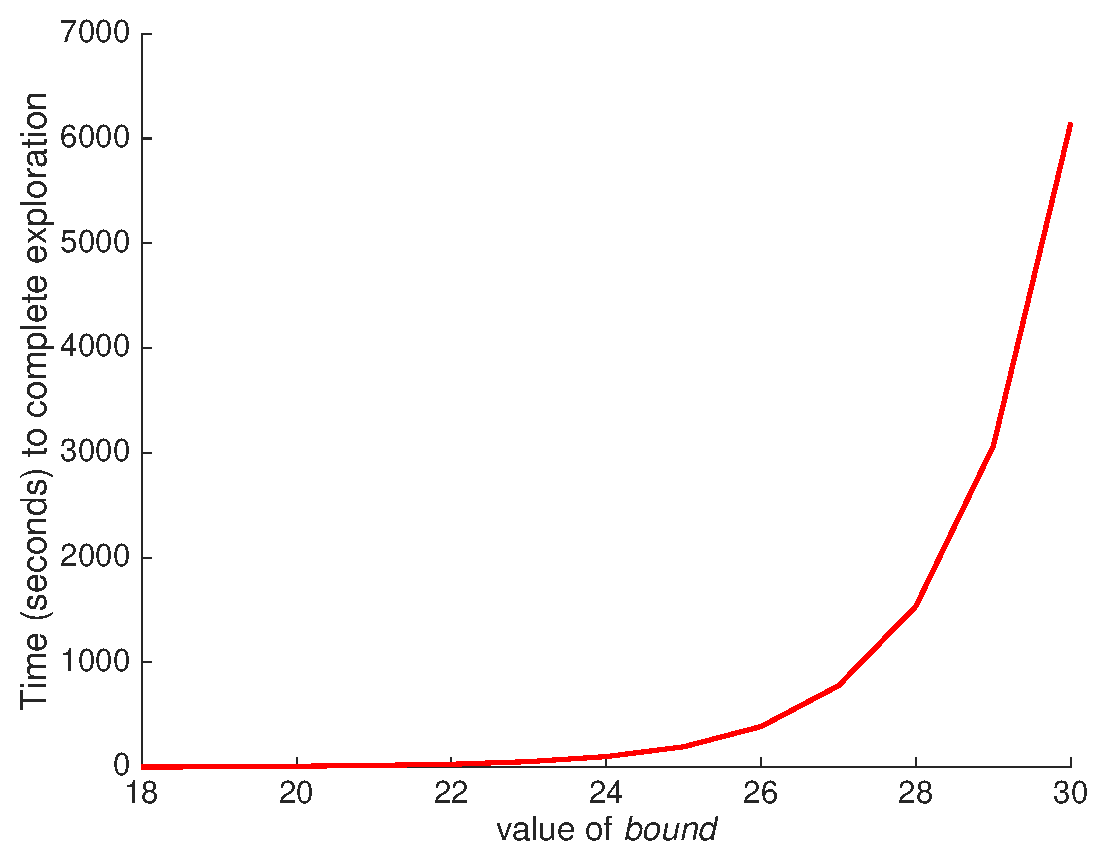
\includegraphics[width=0.4\columnwidth]{figures/sharing_time} }\label{fig:sharing_time}}%
    \qquad
    \subfloat[Maximum memory usage of SPF for covering paths in Listing~\ref{lst:sharing}]{{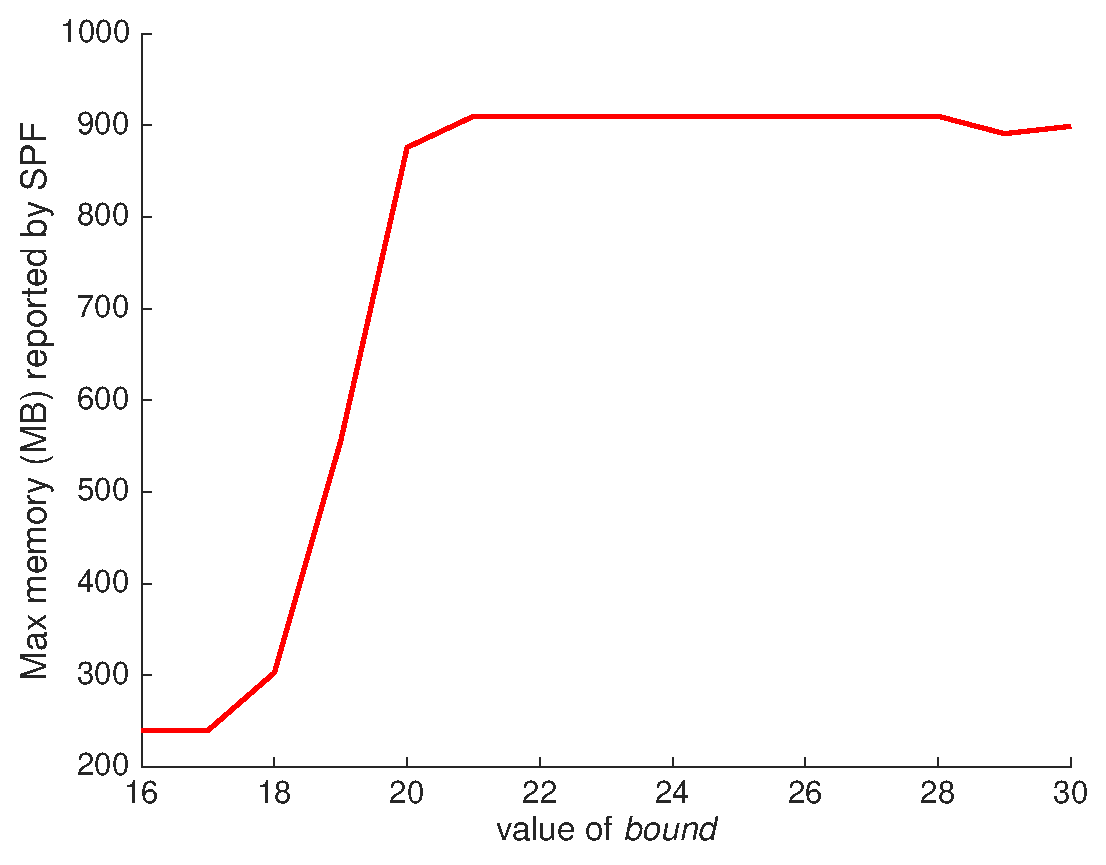
\includegraphics[width=0.4\columnwidth]{figures/sharing_mem} }\label{fig:sharing_mem}}%
    \caption{Time and memory usage of Listing~\ref{lst:sharing} when increasing \textit{bound}}%
    \label{fig:sharing}%
    \vspace{-0.2in}
\end{figure}
%
Figure~\ref{fig:sharing_mem} shows that at a value of 17 for \textit{bound}, the memory usage starts to rise from 240 MB and has reached 910 MB when \textit{bound} equals 21.
%
We also observed that the number of expression objects undergoes a linear increase with the value of \textit{bound}.
%
These three observations lead us to the hypothesis that while SPF does share expression objects internally, the traversal of such expressions breaks the sharing and causes an increase in time and memory.
%
%The time increase is due to garbage collection once the maximum memory threshold is reached.
%
%Integrating veritesting with SPF to make it scale to industrial-sized code requires resolving such engineering issues.
%
\subsection{Complex Expressions}
%Engineering issue \#2: Need to have complex expressions, talk about how Comparators cannot be used anywhere below the top-level operator
During exploration, SPF creates conjunctions of expressions and adds them to its {\em PathCondition} to determine satisfiability of paths.
%
These expressions are allowed to have a \textit{Comparator}~(a comparison operator such as !=) as the top-level operator; however, comparison and Boolean operators are not allowed in sub-expressions.  Thus, the current set of SPF expressions is insufficiently expressive to represent the disjunctive formulas required for multi-path regions.%, and we are currently refactoring the SPF expression hierarchy to allow for richer expression types.
%
%Because SPF has different classes for different expression types~(\textit{IntegerExpressions}, \textit{RealExpression}), these changes must be made in several different places; we believe that moving forward, the
%
%Thus, integrating veritesting presents a design challenge to allow complex expressions in SPF.
%
% \subsection{Intermediate variables}
% %Engineering issue \#3: Nice to introduce intermediate variables
% %
% During veritesting, symbolic formulas derived from static symbolic execution of a region may involve conditional write operations into other variables.
% %
% It is convenient to have intermediate variables~(one per variable written to in the region) which capture such conditional write expressions during the static symbolic execution.
% %
% Later, at an exit point, the intermediate variables can be written into the original variables written to in the region.
% %
% This allows sub-expressions to be shared, and even simplified, without affecting the original variables from the Java bytecode.
% %
% Smaller formulas written into the region\rq s output variables also makes it easier to debug veritesting of regions.
% %
% However, creation of such intermediate variables presents a design challenge in SPF.
% %
% SPF stores and propagates symbolic information through attribute objects.
% %
% This, in turn, creates an invariant that every symbolic variable in the path expression needs to be mapped to an attribute object.

%
%
% \subsection{Veritesting with Multi-threading}
% Veritesting requires SPF to be able to perform static symbolic execution on a region of code and incorporate it as a disjunctive predicate into its path expression along with the corresponding updates to its symbolic store.
% %
% If the region being statically analyzed can be executed in a multi-threaded context, however, then it is necessary to consider all possible points of interference in the region.
% %
% This consideration requires changes to the updates made to SPF\rq s path expression and its symbolic store.
% %
% One way to handle this is to turn every point of interference as an exit point, but determining the possible points of interference statically is itself a difficult problem.  Likely it will require some level of dynamic analysis to determine the points of interference at the time of creation of a veritesting region.
% %
% %But, veritesting would be beneficial if its static analysis also includes computation of points at which interference is infeasible.
% %
% This makes creating an efficient veritesting approach challenging since the cost of this computation must be less than the cost of doing plain dynamic symbolic execution.
















% Data from perl script-based static analysis
% this script just counted the difference between instructions
%
% \begin{table}[]
% \centering
% \caption{My caption}
% \label{my-label}
% \begin{tabular}{|l|l|l|l|}
% \hline
%         & if-ret & if-IV & if-throw \\ \hline
% Chart   & 8.08   & 5.79  & 6.10     \\ \hline
% Closure & 7.40   & 4.37  & 12.6     \\ \hline
% Lang    & 6.3    & 5.23  & 8.26     \\ \hline
% Math    & 12.9   & 6.9   & 9.09     \\ \hline
% Mockito & 8.5    & 4.38  & 11.39    \\ \hline
% Time    & 9.0    & 5.56  & 9.3      \\ \hline
% \end{tabular}
% \end{table}

\section{Related Work}

Path explosion is a major cause of scalability limitations for
symbolic execution, so an appealing direction for optimization is to
combine the representations of similar execution paths, which we refer
to generically as {\em path merging.}
%
If a symbolic execution tool already concurrently maintains objects
representing multiple execution states, a natural approach is to merge
these states, especially ones with the same control-flow location.
%
Hansen et al.~\cite{HansenSS2009} explored this technique but found
mixed results on its benefits.
%
Kuznetsov et al.~\cite{kuznetsov} developed new algorithms and
heuristics to control when to perform such state merging profitably.
%
A larger departure in the architecture of symbolic execution systems
is the MultiSE approach proposed by Sen et al.~\cite{multise}, which
represents values including the program counter with a two-level
guarded structure, in which the guard expressions are optimized with
BDDs.
%
The MultiSE approach achieves effects similar to state merging
automatically, and provides some architectural advantages such as in
representing values that are not supported by the SMT solver.

Another approach to achieve path merging is to statically summarize
regions that contain branching control flow.
%
This approach was proposed by Avgerinos et al.~\cite{veritesting} and
dubbed ``veritesting'' because it pushes symbolic execution further
along a continuum towards all-paths techniques used in verification.
%
A veritesting-style technique is a convenient way to add path merging
to a symbolic execution system that maintains only one execution
state, which is one reason we chose it when extending SPF.
%
Avgerinos et al. implemented their veritesting system
MergePoint to apply binary-level symbolic execution for
bug finding.
%
They found that veritesting provided a dramatic performance
improvement, allowing their system to find more bugs and have better
node and path coverage in a given exploration time.
%
The static regions used by MergePoint are intra-procedural, but they
can have any number of ``transition points'' at which control can be
returned to regular symbolic execution.
%
Avgerinos et al. do not provide details about how MergePoint
represents memory accesses or integrates them with veritesting, though
since MergePoint was built as an extension of the same authors' Mayhem
system, it may reuse techniques such as symbolic representation of
loads from bounded memory regions~\cite{mayhem}.

The veritesting approach has been integrated with another binary level
symbolic execution engine named {\tt angr}~\cite{angr}.
%
However angr's authors found that their veritesting implementation did
not provide an overall improvement over their dynamic symbolic
execution baseline: though veritesting allowed some new crashes to be
found, they observed that giving more complex symbolic expressions
slowed down the SMT solver enough that total performance was degraded.
%
We have also observed complex expressions to be a potential cost of
veritesting, but we believe that optimizations of the SMT solver
interface and potentially heuristics to choose when to use static
regions can allow them to be a net asset.

The way that \tool\ and similar tools statically convert code
regions into formulas is similar to techniques used in verification.
%
In the limit where all relevant code in a program can be
summarized, such as with WBS and TCAS in Section~\ref{sec:results},
\tool\ performs similarly to a bounded symbolic model checker for
Java.
%
SPF and \tool\ build on Java Pathfinder (JPF)~\cite{jpf}, which is
widely used for explicit-state model checking of Java and provides
core infrastructure for instrumentation and state backtracking.
%
Another family of Java analysis tools that use formula translation
(also called verification condition generation) are
ESC/Java~\cite{FlanaganLLNSS2002}, ESC/Java2~\cite{CokK2004}, and
OpenJML~\cite{Cok2011}, though these tools target static error
checking and verification of annotated specifications.

Perhaps the most closely related Java model checking tool is
JBMC~\cite{CordeiroKKST2018}, which has recently been built sharing
infrastructure with the similar C tool CBMC.
%
JBMC performs symbolic bounded model checking of Java code,
transforming code and a supported subset of the standard library into
SMT or SAT formulas that represent all possible execution paths.
%
(The process by which JBMC transforms its internal code representation
into SMT formulas is sometimes described as (static) symbolic
execution, but it has more in common with how \tool\ constructs static
regions than with the symbolic execution that vanilla SPF performs.)
%
In cases that \tool\ can completely summarize, we would expect its
performance to be comparable to JBMC's; an experimental comparison is
future work.
%
But static region summaries are more important as an optimization to
speed up symbolic execution on software that is too large and/or
complex to be explored exhaustively.

A wide variety of other enhancements to symbolic execution have been
proposed to improve its performance, including caching and simplifying
constraints, summarizing repetitive behavior in loops, heuristic
guidance towards interesting code, pruning paths that are repetitive
or unproductive, and many domain-specific ideas.
%
A recent survey by Baldoni et. al.~\cite{SurveySymExec-CSUR18}
provides pointers into the large literature.
%
One approach that is most related to our higher-order static regions
is the function-level compositional approach called SMART proposed by
Godefroid~\cite{Godefroid2007}.
%
Like \tool's function summaries, SMART summarizes the behavior of a
function in isolation from its calling context so that the summary can
be reused at points where the function is used.
%
But SMART uses single-path symbolic execution to compute its
summaries, whereas \tool\ uses static analysis: this makes \tool's
summary more compact at the expense of requiring more reasoning by the
SMT solver.
%
Because SMART was implemented for C, it does not address dynamic
dispatch between multiple call targets.


% %Talk about other symbolic execution performance improvements.
% %mentioned in Christopher Kruegel's ISSTA keynote talk as Static Analysis support
% Other static analysis techniques also provide support for dynamic symbolic execution.
% %
% Loop-extended symbolic execution introduced partial loop summarization by having symbolic variables that represent the number of times each loop executes.
% %
% This technique allowed symbolic variables to incorporate loop dependent effects along with data dependencies from program inputs.
%
%Value Set Analysis~\cite{vsa} is another static analysis technique that can potentially benefit dynamic symbolic execution.
%%
%Value set analysis uses an abstract domain to find an over-approximated set of values that registers or abstract locations may have at program points.
%%
%Value set analysis can help dynamic symbolic execution resolve ranges without solving constraints.
%VSA can resolve ranges without solving constraints, thereby, finding applications in computing all possible write targets during a memory write operation.
%Code summarization (Dodo)
%  - automatically (and statically) summarize effect of loops / functions
%VSA - value set analysis
%  - resolve ranges (and conditionals) without solving constraints

%Talk about TamiFlex, and how using the same technique as TamiFlex is one way to solve veritesting challenges in Java bytecode.
%
%Other techniques for static analysis at the Java bytecode level can also benefit dynamic symbolic execution.
%
%Finding which reflective method call is being used, or handling dynamic class loading are known problems for static analysis tools.
%
%TamiFlex~\cite{tamiflex} provides an answer that is sound with respect to a set of previously seen program runs.
%
%Integrating veritesting runs into similar problems, and using techniques from TamiFlex would allow static predicate construction beyond exit points caused by reflection or dynamic class loading. 

\section{Technique}
%
To add path merging to SPF, we first pre-compute static summaries of arbitrary code regions with more than one execution
path and we also pre-compute method summaries.
%
To bound the set of code regions we analyze, we start by specifying a method $M$ in a configuration file.
%
Next, we construct a set containing only the class $C$ that contains $M$.
%
We then get another set of classes, $C'$,
such that every class in $C'$ has at least one method that was called by a method in a class in $C$.
%
This step which goes from $C$ to $C'$ discovers all the classes at a call depth of 1 from $C$.
%
We continue this method discovery process up to a call depth of 2.
%
While we can increase the call depth in our method discovery process, we found that summarizing
arbitrary code regions with more than 2 calls deep, did not lead to practically useful region summaries.
%
After obtaining a list of methods, we computed static summaries of regions in these methods and method summaries as
explained in Section \ref{sec:static-analysis}.
%
After computing static region and method summaries, we process them as a sequence of transformations described in the next section~\ref{sec:instantiationTransformations} and summarized
in Figure~\ref{fig:overview}.
%
\begin{figure*}[]
    \caption{Overview of transformations on Ranger IR to create and instantiate multi-path region summaries with higher-order regions}
    \label{fig:overview}
    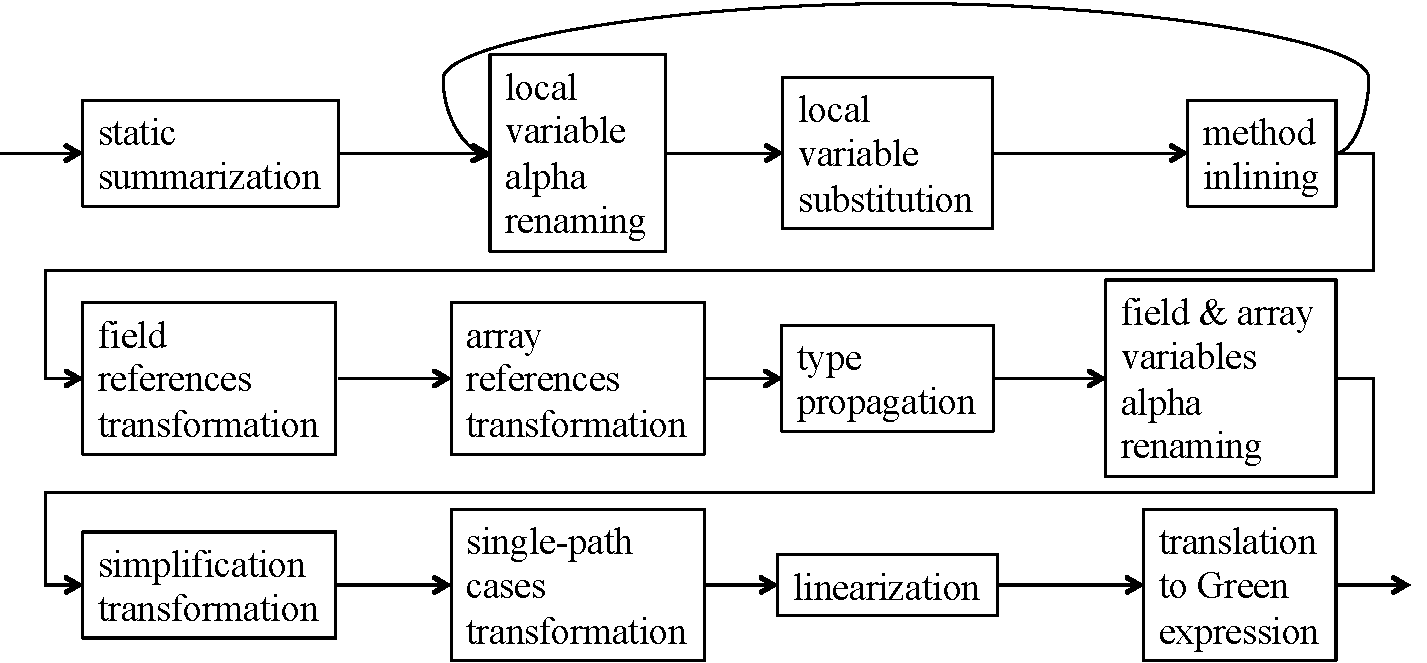
\includegraphics[width=\textwidth]{figures/overview.pdf}
\end{figure*}
%
%
%\subsection{WALA-based analysis for veritesting}
%%
%Veritesting requires static construction of
%predicates of a multi-path region which represent changes to the path expression of the dynamic
%symbolic executor.
%%
%It also requires construction of a control-flow graph of method bodies
%from Java bytecode and finding exit points of the region, which in turn
%requires creation of a control-flow graph of the region.
%%
%Implementing veritesting is made simpler by using a static single
%assignment~(SSA)~\cite{ssa} representation of the multi-path region.
%%
%Using an SSA form allows us to use the $\phi$-expressions created by the
%SSA form and translate them into points at the end of the veritesting
%region where updates to system state along different paths in the region
%can be merged.
%%
%\mike{MWW: Vaibhav please update to describe WALA}
%WALA~\cite{} is a static analysis framework for Java programs that
%has both these features, with
%ExceptionalUnitGraph~\cite{exceptionalunitgraph} and the Shimple
%IR~\cite{shimple}.
%%
%For simple regions with only one exit point, like the one presented in Listing~\ref{lst:v_ex}, we
%were able to use Soot to automate static construction of the predicate representing
%an update to the expression.
%%
%For doing this, we used nodes with more than one successor as the
%starting point, found the immediate post-dominator of the starting
%point, and traversed the control-flow graph on all sides of such branches.
%%
%During such a traversal, we constructed predicates representing the
%multi-path region, similar to the ones presented in
%Listing~\ref{lst:v_ex_smt2}.
%%
%As explained in Section~\ref{sec:exit_points}, including virtual
%function invocations in the construction of our predicates amplifies the
%benefits of veritesting even further.
%%
%We plan to automate this inclusion in the future using Soot.
%%
%Providing SPF with updates to be made to its symbolic store also
%requires Soot to maintain stack location information for variables.
%%
%We plan to automate SPF\rq s symbolic store updates using Soot in the
%future.
%%
%

\subsection{Statement Recovery}
\label{sec:static-analysis}
%Java Ranger has its own AST that captures the statement of regions.
%%
%The choice of having a separate AST for Java Ranger, enables the integration of Java Ranger with any static analysis framework by implementing the transformation that transforms the CFG of a given IR into the corresponding Java Ranger AST representation. 
%%
%We call this interface \textit{Statement Recovery} transformation. \\
%%
%In this transformation we visit nodes in topological order by walking normal edges of a branching points until a \textit{minimum convergent node} is encountered. We define a minimum convergent node as the last immediate successor of blocks following a branching node.
%%
%Note that exceptional edges are ignored during this transformation, however exceptional behavior is later identified and handled through the single path cases.
%%
%We discuss more about this in section~\ref{sec:instantiationTransformations}.
%%
%There are two other things that this transformation takes care of: recovering of complex if-then-else and construction of Gated Single Assignment (GSA).
%%
%Recovering of complex conditions in an if-statement restores its form in the source code. 
%% 
%This is done by identifying \textit{immediate self-contained subgraphs}, that is, subgraphs where the initial node is immediately pre-dominated by the initial node and for the static region and whose successor nodes (up to the region terminus) are dominated (not necessarily immediately) by the initial node.
%%
%
%Construction of Gated Single Assignment (GSA) on the other hand is done by keeping track of the current "conditional path" during translation. More precisely this is done by keeping a stack of  {\tt(Expression x enum \{Then, Else\})} pairs. 
%%
%In addition to that, for each edge between blocks in the block structure, the associated "conditional path" is recorded.  
%%
%So the type of this map (the blockConditionMap) is: {\tt(ISSABasicBlock x ISSABasicBlock) --> List of (Expression x enum \{Then, Else\})}.
%%
%Finally creation of the condition of GSA is done during translating a phi-instruction its immediate predecessor blocks are retrieved then we look up  the edges in the blockConditionMap.  From here, and using condition stack leading to that branch, an if/then/else statement is constructed.

The regions of interest for our technique are bounded by the branch and meet of a given acyclic subgraph.  The intuition is that path explosion during execution of loops is driven by conditional logic within the loop, rather than the loop itself.
Starting from an SSA form, the first transformation recovers a tree-shaped AST for the subgraphs of interest.  While this step is not strictly necessary, it substantially simplifies subsequent transformations.  

The algorithms are similar to those used for those used for decompilation~\cite{Yakdan15@decompilation} but with slightly different goals: 
\begin{itemize}
    \item The algorithm must be {\em accurate} but need not be {\em complete}.  That is, obfuscated regions of code need not be translated into a tree form.
    \item The algorithm must be {\em lightweight} in order to be efficiently performed during analysis.  Thus, algorithms that use global fixpoint computations are 
        too expensive to be used for our purposes.
\end{itemize}

Starting from an initial SSA node, the algorithm first finds the immediate post-dominator of all {\em normal} control paths, that is, paths that do not end in an exception or return instruction.  It then looks for nested self-contained subgraphs.  If for any graph, the post-dominator is also a predecessor of the node, we consider it a loop and discard the region.  

The algorithm systematically attempts to build regions for every branch instruction, even if the branch is already contained within another region.  The reason is that it may not be possible to instantiate the larger region depending on whether summaries can be found for {\em dynamically-dispatched} functions, and whether references are {\em uniquely determinable} for region outputs.

\iffalse
\begin{verbatim}

stmt ::= stmt ; 
   

\end{verbatim}

\vaibhav{assigned to Mike}
\mike{MWW: - we should provide an AST of the constraint language}
\fi 

\subsection{Region Definition}

Once the statement of a multi-path region has been recovered, its corresponding environment is populated.
%
This includes identifying region boundary and creating local variable inputs, outputs, type, and stack slot tables for
the region.
%
The region boundary is used to identify boundaries of the region w.r.t local variables.
%
This is used later to constrain the computation and population of Ranger IR environment tables.
%
For example, the local variable input table is populated with first \textit{use} in the region boundary that map to a given stack slot.
%
The output table is populated with the last \textit{def} of a local variable at merge point of the region.
%
The local variable type table is populated for all variables that lay within the boundaries of the region, this is initially done by
inquiring the static analysis framework, WALA~\cite{Wala} but is later changed by inferring types of local variables
at instantiation and during type propagation transformation~\ref{sec:instantiationTransformations}.

We also construct a stack slot table as part of a region\rq s Ranger IR summary.
%
The stack slot table maps Ranger IR variables to a stack slot, if they correspond to a local variable in the source code.
%
We populate the stack slot table by obtaining a variable to stack slot mapping from WALA.
%
We also assume that, if at least one variable used in a $\phi$-expression is a local variable, then all variables
used in that $\phi$-expression must belong to the same stack slot.
%
We use this assumption to further propagate stack slot information in the stack slot table across all $\phi$-expressions
encountered at merge points of regions.

%The stack slot table on the other hand, does not use region boundary for its population. The reason for this is that,
%the static analysis framework we use, WALA, sometime does not provide information about the stack slots of intermediate
%variables.
%%
%This is particularly problematic in our case because the def of a phi is both an intermediate variable, and so we do
%not know its stack slot, yet it is also an output of the region for which we want to populate its symbolic
%representation onto the stack slot.
%%
%Therefore, our stack slot table uses stack slot inference by propagating the stack slots of vars used in a phi onto the
%def of the phi.
%%
%This requires visiting all variables and phi statements of the IR to maximize the inference of the stack slot, this is
%repeatedly done until a fix point is reached.


\subsection{Instantiation-time Transformations}
\label{sec:instantiationTransformations}

\textbf{Renaming Transformation}: In Alpha renaming transformation, all Ranger IR variables are renamed to ensure their uniqueness before further processing takes place. 
%
This is particularly important not only to ensure uniqueness of variables among different regions, but also to ensure
uniqueness of variable names of the \textit{same} region which might be instantiated multiple times on the same path,
i.e., a region inside a loop will be instantiated multiple times.\\
%
\textbf{Local Variable Substitution Transformation}: During this transformation we eagerly bring in all dynamically
known constant values, symbolic values and references from stack slots into the region for further processing. \\
%
\textbf{Higher-order Regions Transformation}: This transformation is initiated when a method invocation is encountered
during local variable substitution.
%
At this point, we perform three steps.
%
(1) the region that corresponds to the called method is retrieved and alpha renaming of
Ranger IR variables corresponding to local variables is applied on it.
%
(2) Ranger IR expressions that correspond to the actual parameters are evaluated and used to substitute the formal
parameters by repeatedly applying local variable substitution transformation over the method region.
%
(3) When no more higher-order regions can be inlined, the resulting substituted method region is inlined into
the outer region.\\
%
If the method region has a single return value, then the original method invocation is replaced with an assignment to
the returned expression.
%
%Otherwise, inlining of the method region takes place.
%
We dont currently support instantiation of method regions with multiple return statements, support for which requires
another transformation that we talk about in Section~\ref{sec:future}.
\\
\textbf{Field References SSA form}: The field references transformation translates reads and writes of fields
in Java bytecode into corresponding Ranger IR statements.
%
In order to translate all field accesses to SSA form, this transformation creates a summary of the semantics
represented by the field accesses in the region.
%
This transformation constructs a new field access variable for every field assignment on every path within the region.
%
This new field access variable construction makes use of two monotonically increasing subscripts.
%
It uses a path subscript to distinguish between assignments to the same field on the same execution path.
%
It uses a global subscript to distinguish between assignments to the same field across execution paths.
%
At the merge point of the region, field assignments done on the same field are merged using
Gated Single Assignment (GSA)~\cite{Ottenstein1990}.
%
Each merged field access variable has its own path and global subscripts and represents the output of the region into
its field.
%
The path subscript helps us resolve read-after-write operations on the same execution path and find the latest write
into a field on an execution path.
%
The global subscript helps us distinguish between field accesses across multiple execution paths. \\
\textbf{Array References SSA form}: The array references transformation translates reads and writes of arrays in
Java bytecode into corresponding Ranger IR statements.
%
In order to translate all array accesses to SSA form, this transformation creates an execution path-specific copy of
every array when it is first accessed within a region.
%
Reads and writes of arrays are then done on a path-specific copy of the array.
%
All array copies are merged at the merge point of multi-path regions.
%
The merged array copy represents array outputs of the region.\\
\textbf{Type Propagation}: Ranger IR needs to have type information for its variables so that it can construct
corresponding correctly-typed Green variables during the final transformation of the region summary to a Green formula.
%
Having accurate type information is also important for looking up the correct higher-order method summary.
%
As part of region instantiation, Java Ranger infers types of Ranger IR variables in the region summary by
using JPF's runtime environment.
%
Types of local variables are inferred during the local variable substitution transformation and types of field reference
and array reference variables are inferred during their respective transformations.
%
Using these inferred types, the type propagation transformation propagates type information across assignment
statements, binary operations, and variables at leaf nodes of $\gamma$ functions.\\
%
\textbf{Simplification of Ranger IR}: The Ranger IR constructed by earlier transformations computes exact semantics
of all possible behaviors in the region.
%
Representation of such semantics as a formula can often lead to unnecessarily large formulas, which has the potential to
reduce the benefits seen from path merging~\cite{angr}.
%
For example, if an entry in an array is never written to inside a region, the array reference transformation can still have an
array output for that entry that writes a new symbolic variable into it.
%
The region summary would then need to have an additional constraint that makes the new symbolic variable equal the
original value in that array entry.
%
Such conjuncts in the region summary can be easily eliminated with constant propagation, copy propagation, and constant
folding~\cite{dragon-book}.
%
Ranger IR also has statement and expression classes that use a predicate for choosing between two statements (similar to
an {\tt if} statement in Java) and two sub-expressions (similar to the C ternary operator) respectively.
%
When both choices are syntactically equal, the predicated statement and expression objects can be substituted with the
statement or expression on one of their two choices.
%
Such statements and expressions were simplified away to use one of their two choices.
%
Ranger IR performs these two simplifications on such predicated statements and expressions along with constant folding,
constant propagation, and copy propagation.\\
\textbf{Single Path Cases}: This transformation collects path predicates inside a region that lead to
\textit{non-nominal} exit point.
%
This is an alternative approach to that was presented in \cite{veritesting}.
%
In our work we define non-nominal exit point to be points inside the region that either define exceptional behavior or
involve behavior that we cannot summarize, i.e, object creation and throw instructions.
%
The intuition here is that, we want to maximize regions that Java Ranger can summarize, even if the summarization is
only partial.
%
We use this pass of transformation to identify such points, collect their path predicates and prune them away from the
Ranger IR statement.
%
The outcome of this process, is a more simplified and concise statement that represent the nominal behavior of the Ranger region.
%
The collected predicate is later used to guide the symbolic execution to explore non-nominal paths, which Java Ranger
had not summarized.  \\
%
\textbf{Linearization}:
Ranger IR contains translation of branches in the Java bytecode to if-then-else statements defined in the Ranger IR.
%
But the if-then-else statement structure needs to be kept only as long as we have more GSA expressions to be
introduced in the Ranger IR.
%
Once all GSA expressions have been computed, the Ranger IR need not have if-then-else statements anymore.
%
The $\gamma$ functions introduced by GSA are a functional representation of branching, which lets us
capture the semantics of everything happening on both sides of the branch.
%
Since the linearization transformation is done after every field and array entry has been unaliased and converted to
GSA, dropping if-then-else statements from the Ranger IR representation of the region summary reduces redundancy in its
semantics and converts it into a stream of GSA and SSA statements.\\
\textbf{Translation to Green}:
%
At this point Ranger region contains only compositional statements as well as assignment statements that might contain GSA expressions in them.
%
This transformation starts off by translating Ranger variables to Green variables of the right type using the region type table.
%
Then Ranger statements are translated. More precisely, compositional statements are translated into conjunction, assignment statements are translated into Green equality expressions.
%
For assignment statements that have GSA expressions, these are translated into two disjunctive formulas that describes the assignment if the GSA condition or its negation were satisfied. 

\subsection{Checking Correctness Of Region Summaries}
The Ranger IR computed as a result of performing the transformations described in Figure~\ref{fig:overview} should
correctly represent the semantics of the summarized region.
%
If it does not, then using the instantiated region summary can cause symbolic exploration to explore the wrong behavior
of the subject program.
%
We checked the correctness of our instantiated region summaries by using equivalence-checking as defined by Ramos et al.~\cite{ramos}.
%
We designed a test harness that first executes the subject program with a set of symbolic inputs using SPF and
capture the outputs of the subject program.
%
Next, the test harness executes the same subject program with the same set of symbolic inputs using Java Ranger and
capture the outputs of the subject program once again.
%
Finally, the test harness compares outputs returned by symbolic execution with SPF and Java Ranger.
%
If the outputs do not match, then a region summary used by Java Ranger did not contain all the semantics
of the region it summarized.
%
We symbolically execute all execution paths through this test harness.
%
If no mismatch is found between outputs on any execution path, we conclude that all region summaries used by Java Ranger
must correctly represent the semantics of the regions they summarized.
%
We performed correctness-checking on all results reported in this paper.

%\section{Experiments}

\section{Evaluation}
\label{sec:results}
\subsection{Experimental Setup}
We implemented the above mentioned transformations as a wrapper around the Symbolic PathFinder~\cite{spf} tool.
%
To make use of region summaries in Symbolic PathFinder, we use an existing feature of SPF named \textit{listener}.
%
A listener is a method defined within SPF that is called for every bytecode instruction executed by SPF.
%
Java Ranger adds a path merging listener to SPF that, on every instruction, checks (1) if the instruction involves
checking a symbolic condition, and (2) if Java Ranger has a pre-computed static summary that begins at that
instruction\rq s bytecode offset.
%
If both of these conditions are satisfied, Java Ranger instantiates the multi-path region summary corresponding to that
bytecode offset by reading inputs from and writing outputs to the stack and the heap.
%
It then conjuncts the instantiated region summary with the path condition and resumes symbolic execution at the
bytecode offset of the end of the region.
%
Our implementation, named Java Ranger, wraps around SPF and can be configured to run in four modes.
%
(1) In mode 1, it runs vanilla SPF without any path merging enabled.
%
(2) In mode 2, it summarizes multi-path regions only and instantiates them if they are encountered.
%
(3) In mode 3, it summarizes and instantiates methods, by utilizing high ordder regions, along with multi-path regions
as done in mode 2.
%
(4) In mode 4, it uses single-path cases along with multi-path region and method summaries used in mode 3.
%
\subsection{Evaluation}
%\begin{table}[]
    \centering
    \begin{tabular}{|c|c|c|c|c|}
        \hline
        \begin{tabular}[c]{@{}c@{}}Benchmark\\ name\end{tabular} & \begin{tabular}[c]{@{}c@{}}Static analysis\\ time (msec)\end{tabular} & \begin{tabular}[c]{@{}c@{}}\# regions\\ summarized\end{tabular} & \begin{tabular}[c]{@{}c@{}}\# methods\\ summarized\end{tabular} & \begin{tabular}[c]{@{}c@{}}max. branch\\ depth\end{tabular} \\ \hline
        WBS                                                      & 13118                                                                 & 3507                                                            & 2203                                                            & 5                                                           \\ \hline
        TCAS                                                     & 13830                                                                 & 3505                                                            & 2209                                                            & 4                                                           \\ \hline
        Replace                                                  & 7020                                                                  & 119                                                             & 11                                                              & 10                                                          \\ \hline
    \end{tabular}
    \caption{Results of applying our static analysis on a few benchmarks}
    \label{table:static-analysis}
\end{table}
% Please add the following required packages to your document preamble:
% \usepackage{booktabs}
\begin{table}[]
    \begin{tabular}{@{}ccccccccc@{}}
        \toprule
        \begin{tabular}[c]{@{}c@{}}Bench\\ mark\\ Name\end{tabular} & \begin{tabular}[c]{@{}c@{}}Java\\ Ranger\\ mode\end{tabular} & \begin{tabular}[c]{@{}c@{}}\# \\ exec\\ paths\end{tabular} & \begin{tabular}[c]{@{}c@{}}run\\ time\\ (msec)\end{tabular} & \begin{tabular}[c]{@{}c@{}}\# \\ solver\\ queries\end{tabular} & \begin{tabular}[c]{@{}c@{}}solver\\ time\\ (msec)\end{tabular} & \begin{tabular}[c]{@{}c@{}}\# \\ inst.\\ regs\end{tabular} & \begin{tabular}[c]{@{}c@{}}\# \\ inst.\\ methods\end{tabular} & \# inst. \\ \midrule
        WBS-1step                                                   & 1                                                            & 24                                                         & 273                                                         & 46                                                             & 53                                                             & 0                                                          & 0                                                             & 0        \\ \midrule
        WBS-1step                                                   & 2                                                            & 1                                                          & 548                                                         & 0                                                              & 0                                                              & 6                                                          & 0                                                             & 6        \\ \midrule
        WBS-1step                                                   & 3                                                            & 1                                                          & 582                                                         & 0                                                              & 0                                                              & 6                                                          & 0                                                             & 6        \\ \midrule
        WBS-1step                                                   & 4                                                            & 1                                                          & 663                                                         & 6                                                              & 65                                                             & 6                                                          & 0                                                             & 6        \\ \midrule
        TCAS-SR-1step                                               & 1                                                            & 392                                                        & 4115                                                        & 2798                                                           & 3792                                                           & 0                                                          & 0                                                             & 0        \\ \midrule
        TCAS-SR-1step                                               & 2                                                            & 18                                                         & 999                                                         & 74                                                             & 428                                                            & 19                                                         & 0                                                             & 107      \\ \midrule
        TCAS-SR-1step                                               & 3                                                            & 1                                                          & 512                                                         & 0                                                              & 0                                                              & 4                                                          & 28                                                            & 4        \\ \midrule
        TCAS-SR-1step                                               & 4                                                            & 1                                                          & 619                                                         & 4                                                              & 72                                                             & 4                                                          & 28                                                            & 4        \\ \midrule
        Replace                                                     & 1                                                            & 1715                                                       & 3470                                                        & 5482                                                           & 2763                                                           & 0                                                          & 0                                                             & 0        \\ \midrule
        Replace                                                     & 2                                                            & 1080                                                       & 3.0E+04                                                     & 1.30E+04                                                       & 2.5E+04                                                        & 17                                                         & 0                                                             & 977      \\ \midrule
        Replace                                                     & 3                                                            & 632                                                        & 3.7E+04                                                     & 10259                                                          & 2.9E+04                                                        & 24                                                         & 113                                                           & 806      \\ \midrule
        Replace                                                     & 4                                                            & 345                                                        & 1.1E+05                                                     & 7020                                                           & 1.0E+05                                                        & 26                                                         & 122                                                           & 501      \\ \midrule \midrule
        TCAS-1step                                                  & 1                                                            & 392                                                        & 4698                                                        & 2798                                                           & 4287                                                           & 0                                                          & 0                                                             & 0        \\ \midrule
        TCAS-2steps                                                 & 1                                                            & 1.5E+05                                                    & 2.2E+06                                                     & 1.1E+06                                                        & 2.1E+06                                                        & 0                                                          & 0                                                             & 0        \\ \midrule
        TCAS-1step                                                  & 4                                                            & 178                                                        & 6848                                                        & 1719                                                           & 5349                                                           & 13                                                         & 0                                                             & 445      \\ \midrule
        TCAS-2steps                                                 & 4                                                            & 3.2E+04                                                    & 1.4E+06                                                     & 3.1E+05                                                        & 1.2E+06                                                        & 13                                                         & 0                                                             & 8.0E+04  \\ \midrule
        TCAS-SR-2steps                                              & 1                                                            & 1.5E+05                                                    & 1.7E+06                                                     & 1.1E+06                                                        & 1.7E+06                                                        & 0                                                          & 0                                                             & 0        \\ \midrule
        TCAS-SR-2steps                                              & 4                                                            & 1                                                          & 643                                                         & 8                                                              & 106                                                            & 4                                                          & 56                                                            & 8        \\ \midrule
        TCAS-SR-3steps                                              & 4                                                            & 1                                                          & 704                                                         & 12                                                             & 116                                                            & 4                                                          & 84                                                            & 12       \\ \midrule
        TCAS-SR-10steps                                             & 4                                                            & 1                                                          & 1087                                                        & 40                                                             & 354                                                            & 4                                                          & 280                                                           & 40       \\ \midrule
        WBS-2steps                                                  & 1                                                            & 576                                                        & 775                                                         & 1150                                                           & 418                                                            & 0                                                          & 0                                                             & 0        \\ \midrule
        WBS-3steps                                                  & 1                                                            & 1.4E+04                                                    & 9806                                                        & 2.8E+04                                                        & 8364                                                           & 0                                                          & 0                                                             & 0        \\ \midrule
        WBS-4steps                                                  & 1                                                            & 3.3E+05                                                    & 2.2E+05                                                     & 6.6E+05                                                        & 1.9E+05                                                        & 0                                                          & 0                                                             & 0        \\ \midrule
        WBS-5steps                                                  & 1                                                            & 8.0E+06                                                    & 5.3E+06                                                     & 1.2E+07                                                        & 4.4E+06                                                        & 0                                                          & 0                                                             & 0        \\ \midrule
        WBS-2steps                                                  & 4                                                            & 1                                                          & 971                                                         & 20                                                             & 401                                                            & 15                                                         & 0                                                             & 20       \\ \midrule
        WBS-3steps                                                  & 4                                                            & 1                                                          & 1344                                                        & 35                                                             & 769                                                            & 16                                                         & 0                                                             & 35       \\ \midrule
        WBS-4steps                                                  & 4                                                            & 1                                                          & 1919                                                        & 50                                                             & 1235                                                           & 16                                                         & 0                                                             & 50       \\ \midrule
        WBS-5steps                                                  & 4                                                            & 1                                                          & 2165                                                        & 65                                                             & 1523                                                           & 16                                                         & 0                                                             & 65       \\ \midrule
        WBS-6steps                                                  & 4                                                            & 1                                                          & 3239                                                        & 80                                                             & 2479                                                           & 16                                                         & 0                                                             & 80       \\ \midrule
        WBS-10steps                                                 & 4                                                            & 1                                                          & 3895                                                        & 140                                                            & 3163                                                           & 16                                                         & 0                                                             & 140      \\ \bottomrule
    \end{tabular}
    \caption{Java Ranger Performance on WBS, TCAS, TCAS-SR, and Replace}
    \label{table:results}
\end{table}
%
In order to evaluate the performance of Java Ranger, we used the following benchmarking programs commonly used to evaluate symbolic
execution performance.
%
(1) Wheel Brake System (WBS)~\cite{yang2014directed} is a synchronous reactive
component developed to make aircraft brake safely when taxing, landing, and during a rejected take-off.
%
(2) Traffic Collision Avoidance System (TCAS) is part of a suite of programs commonly referred to as the Siemens
suite~\cite{siemens-benchmarks}. TCAS is a system that maintains altitude separation between aircraft to avoid mid-air
collisions.
%
(3) Replace is another program that\rq s part of the Siemens suite. Replace searches for a pattern in a given input and
replaces it with another input string.
%
We used the translation of the Siemens suite to Java as made available by Wang et al.~\cite{dgse}.
%
We also manually created a variant of TCAS by converting regions of code with return statements on
every execution path to regions of code with a single return statement at the merge point of the region.
%
We refer to this variant of TCAS as TCAS-SR (TCAS with Single Returns).
%
We also created variants of WBS, TCAS, and TCAS-SR by running them for multiple steps.
%

%We ran WBS, TCAS, TCAS-SR, and Replace using Java Ranger and first report the result of static analysis on these
%three benchmarks in Table~\ref{table:static-analysis}.
%
%The number of static regions summarized for WBS and TCAS is dominated by region summaries found in the Java standard
%library used by WBS and TCAS.
%%
%Replace doesn't use the Java standard library, which is reflect in Table~\ref{table:static-analysis}.
%%
%We also report the most number of branches seen in our static regions with each benchmark.
%%
%Being able to instantiate static summaries of such regions potentially increases the path reduction we get from path-merging.

We ran WBS, TCAS, TCAS-SR, and Replace using Java Ranger and present our results from instantiating region summaries
in Table~\ref{table:results}.
%
Table~\ref{table:results} shows that Java Ranger achieves a significant improvement using path-merging with WBS.
%
The ``\# exec paths'' column is the number of execution paths required to completely explore the benchmark.
%
``runtime (msec)'' is the time taken for dynamic analysis (excludes static analysis time).
%
``\# inst. regs'' is the total number of regions that were instantiated at least once when running each benchmark.
%
``\# inst. methods'' is the number of higher-order regions that were used and ``inst.'' is the total number of
instantiations that was done when running the benchmark.
%
Table~\ref{table:results} shows that we achieve a significant improvement using path-merging with WBS.
%
Java Ranger outperforms SPF when running TCAS too but it doesn't allow path merging to summarize the entire program
to a single execution path, as in the case with WBS.
%
We manually analyzed TCAS and found the only barrier to our path-merging was the presence of several code
regions containing a return instruction on every execution path.
%
We manually performed a semantics-preserving transformation to the source code of TCAS to create another version, TCAS-SR,
that has a single return value at the end of all such multi-path regions.
%
We plan to automate this transformation in the future, see future work section~\ref{sec:futureWork}.
%
Table~\ref{table:results} shows the benefit of such a \textit{multiple-returns-to-single-return} transformation.
%
It allows Java Ranger to summarize the entire TCAS-SR program into a single execution path.
%
This is made possible by the use of higher-order regions as shown in Table~\ref{table:results}.
%
In mode 2, Java Ranger explores 18 execution paths with TCAS-SR, whereas in mode 3~(mode 2 + higher-order region support), it needs to only explore a single
execution path because it can instantiate 28 higher-order method summaries.
%
The bottom half of Table~\ref{table:results} also shows the benefits of path-merging with Java Ranger increase as we run
more steps of WBS, TCAS, and TCAS-SR.
%
We ran as many steps of each of these 3 benchmarks as possible with a 6 hour timeout using Java Ranger in modes
1 (runs Java Ranger without path merging) and 3 (runs Java Ranger with multi-path region summaries and higher-order region summaries).
%
While, in mode 1, Java Ranger can only run 5 steps of WBS in less than 6 hours, in mode 4 (path merging with multi-path regions, higher-order regions, and single-path cases),
Java Ranger can easily execute up to 10 steps in less than 4 seconds.
%
A similar benefit is seen with TCAS-SR where Java Ranger in mode 1 can only run 2 steps of TCAS-SR in 6 hours, but in
mode 4, it can easily run up to 10 steps of TCAS-SR in about 1 second.

However, the performance of Java Ranger when running Replace is quite different from that seen when running WBS, TCAS, and TCAS-SR.
%
While Java Ranger reduces the total number of execution paths with every increase in mode, the path reduction isn't as significant.
%
More importantly, it also makes an order of magnitude more solver calls thereby increasing the total runtime.

We further investigated this drop in performance of Java Ranger when running Replace by exploring the space of potential
regions to instantiate.
%
We obtained the list of regions that are instantiated at least once when running Replace with Java Ranger in mode 3~(using
high order and multi-path region summaries).
%
This step produced a list of 24 regions.
%
Next, we sampled the space of all possible subsets of this set of 24 regions by
%
(1) randomly enumerating the space up to 11500 subsets of all possible subsets of 24 regions,
%
(2) enumerating the space in the order of set size up to all subsets of 3 regions from a set of 24 regions.
%
With both methods of enumeration, we searched for the least amount of time Java Ranger needs to instantiate at least one
region with Replace.
%
We found this least time to be 26.3 seconds which is still more than the 3.47 seconds Java Ranger needs to run
Replace in mode 1 (running vanilla SPF with no path merging).
%
In the fastest runs with at least one region instantiation in both methods of enumeration, Java Ranger finished
exploration with the same number of execution paths as that explored during mode 1.
%
The result of this analysis, combined with a significant increase in the number of solver queries with Java Ranger's
path-merging modes, points toward the conclusion that every instantiation of a multi-path region in Replace causes another branch to be
symbolic.
%
This conclusion is also in alignment with the observation made by Kuznetsov et al.~\cite{kuznetsov} that path merging can
sometimes have a net negative effect on the performance of symbolic execution.
%
We plan to integrate heuristics for estimating the side-effects of introducing new symbolic state as a result of
path merging on symbolic execution performance with Java Ranger in the future.

\section{Future Work}
\label{sec:futureWork}
While Java Ranger has the potential to scale to large real-world Java programs, there are a number of directions along
which it can be further improved.
\begin{itemize}

\item Java Ranger attempts to perform path merging as aggresively as possible. This path merging strategy doesn't
optimize towards making fewer solver calls. We plan to work towards implementing heuristics that
can measure the effect of path merging on the rest of the program.
    
%\item In some models, it is possible to reduce the number of paths to one.  The static region approach essentially
%constructs a unrolled version of the program, similar to what tools like CBMC construct.   This can only happen on
%relatively static models that do not have a lot of object construction leading to multiple dispatch paths.  HOSRs are
%more flexible for these situations and allow specialization depending on dispatch type, which we believe will lead to
%better performance for highly-dynamic models.
%
%\item In general, the solver time does not rise dramatically for disjunctive paths. Since (in the limit) we reduce the
%number of paths exponentially by removing branches, we can perform relatively expensive analyses as preprocessing steps
%and at instantiation if we are able to instantiate a static region, and still end up with much better performance.

\item Java Ranger is most useful when it can merge multiple execution paths into one summary. But such merging causes an
increase in the size of the summary, and consequently, the path condition.
%
Once a summary has been communicated to the solver, it need not be sent again as long as it remains the same.
%
This requires us to use the solver in an incremental mode, where we use previously-constructed state in the solver for
future solving.
%
Our current implementation of Java Ranger sends the entire path condition to the solver with every query, making every
query even more expensive in the presence of large multi-path region summaries.
%
We plan to integrate incremental solving with Java Ranger in the future.
%
\item Multiple return instructions that appear on all execution paths inside a multi-path region can be simplified to a
single return value of the region.
%
We implemented this transformation manually in TCAS but we plan to automate it in the future.
%
Such automation would allow us to summarize regions with return instructions.
%
\item Support of Test Case Generation: while statically summarizing regions gives dynamic symbolic execution a
performance boost to explore more paths efficiently, generating test cases that covers all summarized branches is one of
the fundamental roles of dynamic symbolic execution that is currently unsupported.
%
This is an extension that we intend to investigate in our future work.
%
\item While path merging can potentially allow symbolic execution to explore interesting parts of a program sooner, the
effect of path merging on search strategies, such as depth-first search and breadth-first search commonly used with
symbolic execution, remains to be investigated. We plan to explore the integration of such guidance heuristics with path merging in the future.
%
\item Java Ranger can summarize methods and regions in Java standard libraries. This creates potential for automatically
constructing summaries of standard libraries so that Java symbolic execution engines can prevent path explosion
originating from standard libraries.
%
\end{itemize}
\section{Conclusion}
\vaibhav{assigned to the one who gets to it first}

\mike{Future work: }

Extensions: 
\begin{enumerate}
\item Simplification of static regions at instantiation time using constant propagation, code specialization, etc.

\item Adding support for parallel Java programs with static regions

\item Adaptation of metric-based test-case generation for static regions: statement, branch, MCDC, observable metrics.

\item Parallelization of the analysis process (similar to Staats work in 2011)

\item Adding support for bypass of complex expressions: {\em symcrete} execution involving regions.

\item Integration with the Green constraint solver

\end{enumerate}

Other improvements:
\begin{enumerate}
\item Simplification of the Symbolic PathFinder constraint mechanism

\item Interpolation-based path subsumption checks  (c.f.: "More Effective Interpolations in Software Model Checking" - ASE 2017")

\end{enumerate}




\bibliographystyle{ACM-Reference-Format}
\bibliography{references}
\newpage
\clearpage
\section{Appendix}
\label{sec:appendix}
We report results from our evaluations for each benchmark in Tables~\ref{table:results1} and~\ref{table:results2}
% Please add the following required packages to your document preamble:
% \usepackage{booktabs}
\begin{table}[]
    \begin{tabular}{@{}ccccccccc@{}}
        \toprule
        \begin{tabular}[c]{@{}c@{}}Bench\\ mark\\ Name\end{tabular} & \begin{tabular}[c]{@{}c@{}}Java\\ Ranger\\ mode\end{tabular} & \begin{tabular}[c]{@{}c@{}}\# \\ exec\\ paths\end{tabular} & \begin{tabular}[c]{@{}c@{}}run\\ time\\ (msec)\end{tabular} & \begin{tabular}[c]{@{}c@{}}\# \\ solver\\ queries\end{tabular} & \begin{tabular}[c]{@{}c@{}}solver\\ time\\ (msec)\end{tabular} & \begin{tabular}[c]{@{}c@{}}\# \\ inst.\\ regs\end{tabular} & \begin{tabular}[c]{@{}c@{}}\# \\ inst.\\ methods\end{tabular} & \# inst. \\ \midrule
        WBS-1step                                                   & 1                                                            & 24                                                         & 273                                                         & 46                                                             & 53                                                             & 0                                                          & 0                                                             & 0        \\ \midrule
        WBS-1step                                                   & 2                                                            & 1                                                          & 548                                                         & 0                                                              & 0                                                              & 6                                                          & 0                                                             & 6        \\ \midrule
        WBS-1step                                                   & 3                                                            & 1                                                          & 582                                                         & 0                                                              & 0                                                              & 6                                                          & 0                                                             & 6        \\ \midrule
        WBS-1step                                                   & 4                                                            & 1                                                          & 663                                                         & 6                                                              & 65                                                             & 6                                                          & 0                                                             & 6        \\ \midrule
        TCAS-SR-1step                                               & 1                                                            & 392                                                        & 4115                                                        & 2798                                                           & 3792                                                           & 0                                                          & 0                                                             & 0        \\ \midrule
        TCAS-SR-1step                                               & 2                                                            & 18                                                         & 999                                                         & 74                                                             & 428                                                            & 19                                                         & 0                                                             & 107      \\ \midrule
        TCAS-SR-1step                                               & 3                                                            & 1                                                          & 512                                                         & 0                                                              & 0                                                              & 4                                                          & 28                                                            & 4        \\ \midrule
        TCAS-SR-1step                                               & 4                                                            & 1                                                          & 619                                                         & 4                                                              & 72                                                             & 4                                                          & 28                                                            & 4        \\ \midrule
        Replace                                                     & 1                                                            & 1715                                                       & 3470                                                        & 5482                                                           & 2763                                                           & 0                                                          & 0                                                             & 0        \\ \midrule
        Replace                                                     & 2                                                            & 1080                                                       & 3.0E+04                                                     & 1.30E+04                                                       & 2.5E+04                                                        & 17                                                         & 0                                                             & 977      \\ \midrule
        Replace                                                     & 3                                                            & 632                                                        & 3.7E+04                                                     & 10259                                                          & 2.9E+04                                                        & 24                                                         & 113                                                           & 806      \\ \midrule
        Replace                                                     & 4                                                            & 345                                                        & 1.1E+05                                                     & 7020                                                           & 1.0E+05                                                        & 26                                                         & 122                                                           & 501      \\ \midrule \midrule
        TCAS-1step                                                  & 1                                                            & 392                                                        & 4698                                                        & 2798                                                           & 4287                                                           & 0                                                          & 0                                                             & 0        \\ \midrule
        TCAS-2steps                                                 & 1                                                            & 1.5E+05                                                    & 2.2E+06                                                     & 1.1E+06                                                        & 2.1E+06                                                        & 0                                                          & 0                                                             & 0        \\ \midrule
        TCAS-1step                                                  & 4                                                            & 178                                                        & 6848                                                        & 1719                                                           & 5349                                                           & 13                                                         & 0                                                             & 445      \\ \midrule
        TCAS-2steps                                                 & 4                                                            & 3.2E+04                                                    & 1.4E+06                                                     & 3.1E+05                                                        & 1.2E+06                                                        & 13                                                         & 0                                                             & 8.0E+04  \\ \midrule
        TCAS-SR-2steps                                              & 1                                                            & 1.5E+05                                                    & 1.7E+06                                                     & 1.1E+06                                                        & 1.7E+06                                                        & 0                                                          & 0                                                             & 0        \\ \midrule
        TCAS-SR-2steps                                              & 4                                                            & 1                                                          & 643                                                         & 8                                                              & 106                                                            & 4                                                          & 56                                                            & 8        \\ \midrule
        TCAS-SR-3steps                                              & 4                                                            & 1                                                          & 704                                                         & 12                                                             & 116                                                            & 4                                                          & 84                                                            & 12       \\ \midrule
        TCAS-SR-10steps                                             & 4                                                            & 1                                                          & 1087                                                        & 40                                                             & 354                                                            & 4                                                          & 280                                                           & 40       \\ \midrule
        WBS-2steps                                                  & 1                                                            & 576                                                        & 775                                                         & 1150                                                           & 418                                                            & 0                                                          & 0                                                             & 0        \\ \midrule
        WBS-3steps                                                  & 1                                                            & 1.4E+04                                                    & 9806                                                        & 2.8E+04                                                        & 8364                                                           & 0                                                          & 0                                                             & 0        \\ \midrule
        WBS-4steps                                                  & 1                                                            & 3.3E+05                                                    & 2.2E+05                                                     & 6.6E+05                                                        & 1.9E+05                                                        & 0                                                          & 0                                                             & 0        \\ \midrule
        WBS-5steps                                                  & 1                                                            & 8.0E+06                                                    & 5.3E+06                                                     & 1.2E+07                                                        & 4.4E+06                                                        & 0                                                          & 0                                                             & 0        \\ \midrule
        WBS-2steps                                                  & 4                                                            & 1                                                          & 971                                                         & 20                                                             & 401                                                            & 15                                                         & 0                                                             & 20       \\ \midrule
        WBS-3steps                                                  & 4                                                            & 1                                                          & 1344                                                        & 35                                                             & 769                                                            & 16                                                         & 0                                                             & 35       \\ \midrule
        WBS-4steps                                                  & 4                                                            & 1                                                          & 1919                                                        & 50                                                             & 1235                                                           & 16                                                         & 0                                                             & 50       \\ \midrule
        WBS-5steps                                                  & 4                                                            & 1                                                          & 2165                                                        & 65                                                             & 1523                                                           & 16                                                         & 0                                                             & 65       \\ \midrule
        WBS-6steps                                                  & 4                                                            & 1                                                          & 3239                                                        & 80                                                             & 2479                                                           & 16                                                         & 0                                                             & 80       \\ \midrule
        WBS-10steps                                                 & 4                                                            & 1                                                          & 3895                                                        & 140                                                            & 3163                                                           & 16                                                         & 0                                                             & 140      \\ \bottomrule
    \end{tabular}
    \caption{Java Ranger Performance on WBS, TCAS, TCAS-SR, and Replace}
    \label{table:results}
\end{table}






\end{document}
